% !TEX program = xelatex
\documentclass[b5paper, 11pt, openleft]{memoir}

\usepackage{indentfirst}

%%% Font setup
\usepackage[no-math]{fontspec}
\setmainfont{ZillaSlab}[
    Path = fonts/,
    Extension = .ttf,
    UprightFont = *-Regular,
    ItalicFont = *-Italic,
    BoldFont = *-Bold,
    BoldItalicFont = *-BoldItalic,
    Ligatures = {TeX, Common}
]
\setmonofont[Scale = MatchLowercase]{Iosevka Custom}
\XeTeXlinebreaklocale="en_EN"
\XeTeXlinebreakskip=0pt plus 3pt
\emergencystretch=1em

\usepackage{mathtools}
\usepackage[math-style = ISO, mathrm = sym, warnings-off = {mathtools-colon}]{unicode-math}
\setmathfont[Scale = MatchLowercase]{Concrete-Math.otf}
\noDisplayskipStretch
\setoperatorfont\symscr
\everymath{\displaystyle}

%%% Stylings
% Page Layout and Margins
\setsecnumdepth{subsection}
\settocdepth{subsection}
\setlrmarginsandblock{4cm}{1.5cm}{*}
\setulmarginsandblock{3cm}{2.5cm}{*}
\setlength{\headheight}{30pt}
\setlength{\parindent}{1.5cm}
\setlength{\parskip}{0.3em}
\setlength{\beforechapskip}{20pt}
\renewcommand{\arraystretch}{1}
\allowdisplaybreaks
\setSpacing{1.5}
\checkandfixthelayout

% Footnotes
\usepackage{fancyhdr}
\pagestyle{fancy}
\fancyhead[LE]{\textbf{\thepage ~ $\big\vert$ \leftmark}}
\fancyhead[RO]{\textbf{\rightmark ~ $\big\vert$ \thepage}}
\fancyhead[RE, LO, C]{}

% Styling Figures
\usepackage{multicol, caption}
\setlength{\columnseprule}{1pt}
\def\columnseprulecolor{\color{lightgray}}
\DeclareCaptionLabelSeparator{pipe}{ $\vert$ }
\captionsetup{
    labelfont = {bf},
    font = {small, sc},
    width = 0.6\textwidth,
    labelsep = pipe,
    figurename = \textbf{Fig. }
}

% Styling Titles
\renewcommand{\partnamefont}{\LARGE\bfseries\scshape\centering}
\renewcommand{\partnumfont}{\LARGE\bfseries\scshape\centering\MakeUppercase}
\renewcommand{\midpartskip}{\par\rule{1in}{0.5pt}\vspace{1em}\par}
\renewcommand{\printparttitle}{\HUGE\bfseries\scshape\centering}
\renewcommand{\afterpartskip}{\relax}
\chapterstyle{veelo}
    \renewcommand*{\printchapternum}{%
    \makebox[0pt][l]{%
    \hspace{.8em}%
    \resizebox{!}{\beforechapskip}%
    {\chapnumfont \thechapter}%
    \hspace{.8em}%
    \rule{2\midchapskip}{\beforechapskip}%
    }%
}

% Packages
\usepackage[dvipsnames]{xcolor}
\usepackage{subcaption, graphicx, pdfpages, float, wrapfig}
\graphicspath{{diagrams/}}
\usepackage{minted}
\usemintedstyle{algol_nu}
\setminted{
    frame = lines,
    bgcolor = lightgray,
    linenos,
	breaklines
}
\usepackage{csquotes}
\usepackage[inline]{enumitem}

\usepackage[colorlinks, allcolors = blue]{hyperref}
\usepackage{cleveref}

%%% Mathematical packages 
\usepackage[]{siunitx}
\usepackage{physics2}
\usepackage{derivative}
\usephysicsmodule{ab, ab.braket, ab.legacy, nabla.legacy, op.legacy}
\usepackage[makeroom]{cancel}
% Proofs
\usepackage{amsthm}
\usepackage{tcolorbox}
\tcbuselibrary{breakable, theorems, skins}
\newtcbtheorem[auto counter, crefname = {theorem}{theorems}, Crefname = {Theorem}{Theorems}]{theorem}{Theorem}{
    coltitle = black,
    sharp corners, frame hidden, enhanced, colback = lightgray!10, breakable,
    borderline west = {3pt}{-3pt}{lightgray},
    detach title = true,
    fonttitle = \bfseries, before upper = {\tcbtitle\quad}
}{theorem}
\newtcbtheorem[auto counter, crefname = {axiom}{axioms}, Crefname = {Axiom}{Axioms}]{axiom}{Axiom}{
    sharp corners, colback = lightgray!40, colframe = darkgray, breakable
}{axiom}
\newtcbtheorem[auto counter, crefname = {definition}{definition}, Crefname = {Definition}{Definition}]{df}{Definition}{
    sharp corners, colback = lightgray!40, colframe = darkgray, breakable
}{df}
\newtcbtheorem[auto counter, number within = section]{exmp}{Example}{
    colback = lightgray!40, colframe = darkgray, breakable
}{exmp}
\newtcbtheorem[auto counter, number within = chapter, crefname = {remarks of chapter }{remarks of chapter }, Crefname = {Remarks}{Remarks}]{remark}{Remarks on chapter }{
    colback = lightgray!10, colframe = black, breakable
}{remark}

%%% Mathematical commands
% Geometry
\let\line\overline
% Mathematical constants
\newcommand{\e}{\symrm{e}}
\newcommand{\im}{\symrm{i}}
\newcommand{\cpi}{\symrm{\pi}}
\DeclareMathOperator*{\ssum}{\symrm{\Sigma}}
\DeclareMathOperator*{\Proj}{\symrm{Proj}}
\DeclareMathOperator*{\sgn}{\symrm{sgn}}
% Vector notations
\newcommand{\vv}[1]{\pmb{\symrm{#1}}}
\newcommand{\vdot}{\pmb{\cdot}}
\newcommand{\conj}{^{\ast}}
\newcommand{\dagr}{^{\dag}}
\newcommand{\trnsp}{^{\intercal}}
\newcommand{\iden}{\symbb{I}}
\newcommand{\uv}[1]{\hat{\vv{e}}_{#1}}
\newcommand{\tensor}{\otimes}
\newcommand{\bmat}[1]{
	\begin{bmatrix}
		#1
	\end{bmatrix}
}
\newcommand{\ihat}{\hat{\i}}
\newcommand{\jhat}{\hat{\j}}
\newcommand{\khat}{\hat{k}}
% Differences
\DeclareMathOperator{\kdel}{\symrm{\delta}}
\DeclareMathOperator{\ddel}{\symrm{\delta}}
\newcommand{\Dd}{\symrm{\Delta}}
% Physics quantities symbols
\newcommand{\lagr}{\mathcal{L}}
\newcommand{\haml}{\mathcal{H}}
\newcommand{\hilb}{\mathcal{E}}
% Calculus notations
\newcommand{\appr}{\rightarrow}
\newcommand{\alc}[2][0.3]{&\parbox[c]{#1\textwidth}{#2}}
\newcommand{\pintm}[1]{\mathcal{D}[#1]}
% Mathematical conjunctions and expressions
\newcommand{\mathand}{\quad\textrm{and,}\quad}
\newcommand{\mathor}{\quad\textrm{or,}\quad}
\newcommand{\mathif}{\quad\textrm{if}\quad}
\newcommand{\mathiff}{\quad\textrm{\emph{iff}}\quad}
\newcommand{\maththerefore}{\emquad\textrm{\emph{therefore,}}\emquad}
\newcommand{\ifft}{\emph{iff}}
% Notational commands
\newcommand{\flatfrac}[2]{#1\fracslash#2}
% Column types
\newcolumntype{C}{>{$}c<{$}}
\newcolumntype{L}{>{$}l<{$}}
\newcolumntype{R}{>{$}r<{$}}

%%% Type commands
\newcommand{\conclusion}{\section{Conclusion for Chapter \thechapter}}
\newcommand{\formula}{\section{Formula from Chapter \thechapter}}
\newcommand{\prelude}[1]{
    \chapter*{Prelude: #1}
    \addcontentsline{toc}{chapter}{Prelude: #1}
}
\newcommand{\prerequisites}[1]{\textbf{Prerequisites:}~\emph{#1}}

% Bibliographies
\usepackage[
    backend = biber,
    style = phys,
    sorting = anyvt
]{biblatex}
\addbibresource{bibliography.bib}

% Indices
\usepackage{imakeidx}
\makeindex

\begin{document}

% \thispagestyle{empty}
% 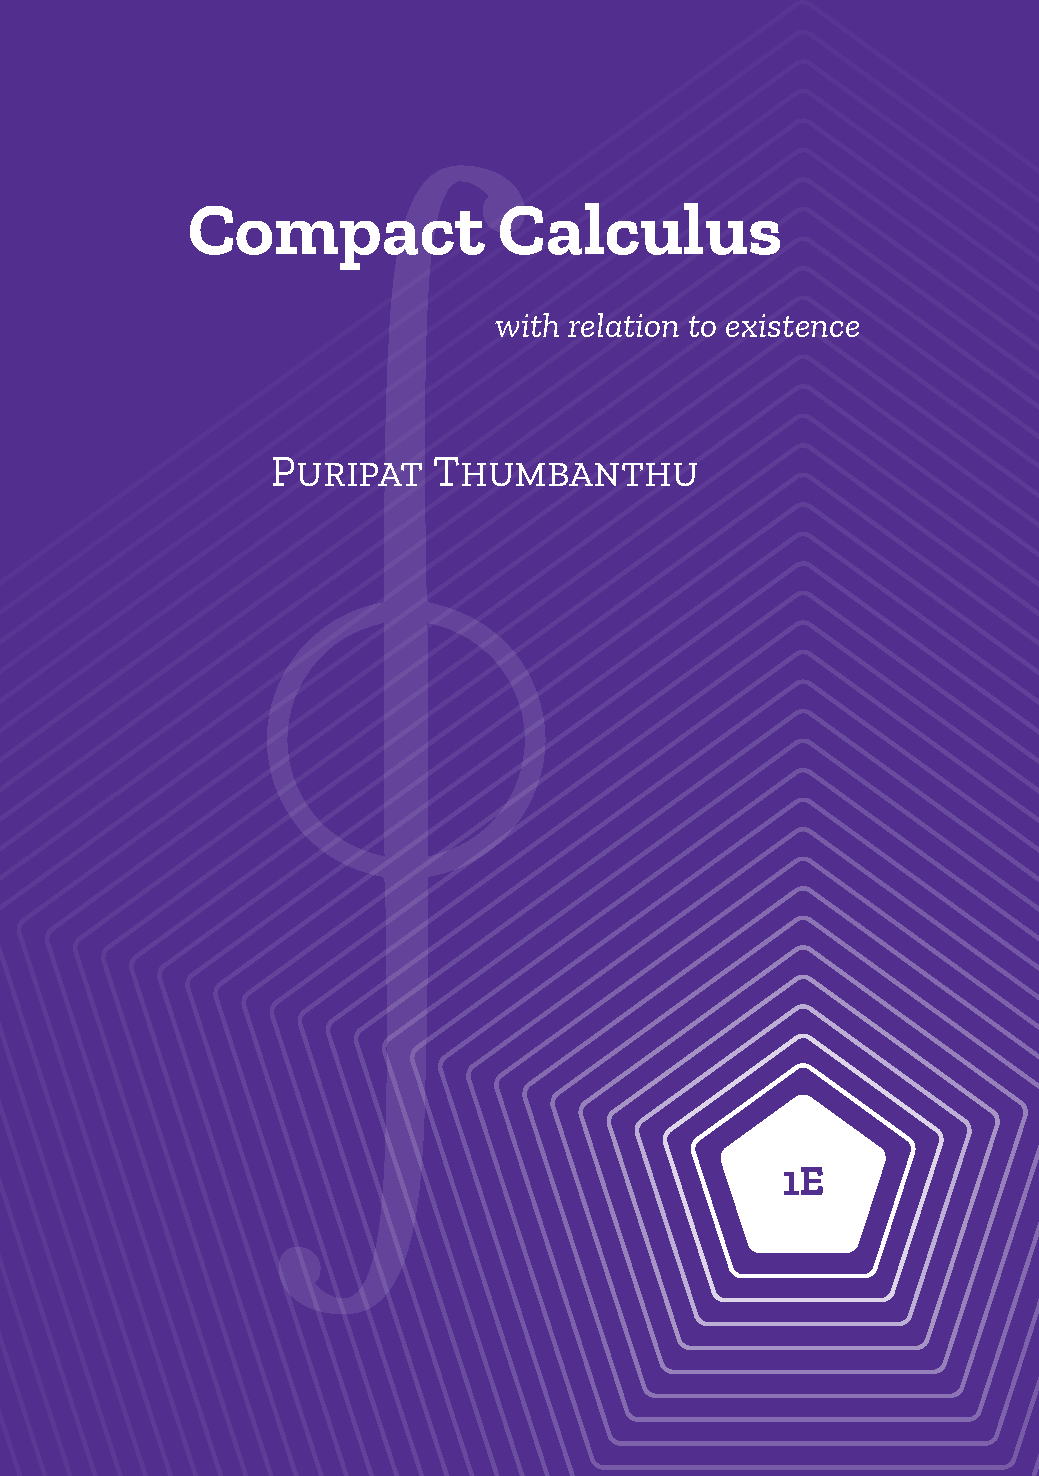
\includepdf{coverpage.pdf}

\thispagestyle{empty}
\title{Compact Calculus - Calculus for the practitioners}
\author{Puripat Thumbanthu, Kunakorn Chaiyara}
\date{Started: 07/28/2022 \\Revision: \today}
\maketitle

\frontmatter

\prerequisites{set theory, algebra, geometry, basic trigonometry}

\tableofcontents*

\chapter*{Preface}
\addcontentsline{toc}{chapter}{Preface}

\section{Purpose of the textbook}

I probably made a lot of mathematicians angry by writing this book. But it misses their points. This textbook is designed for the practitioners of calculus: people that are interested in fields of sciences including biology, chemistry, and physics. Therefore, expect what you aren't expected, and don't expect what you traditionally expect.

The contents of this textbook are entirely self-contained and organized into four parts (volumes)\footnote{The exact number of parts may change as more material is added during the writing process.}: dynamical systems and ordinary differential equations, signal analysis, real and complex analysis, and vector calculus with partial differential equations. However, the topics deviates greatly from the traditional way calculus is taught. I took a great care of how the material is arranged in better needs practitioners, which means it may deviate from a standard calculus curriculum. To maintain focus within the core chapters, the auxilaries topics typically covered in traditional courses have been moved to the appendices.

Even though the book is very self-contained, it still doesn't serve as a standalone book. Sure, the story that I'm about to tell is quite fruitful, and you can enjoy it from the beginning to end. But, it lacks one thing: problem solving experiences. As of the revision today (\today), there are not that many exercises in the chapters. So, you might have to find some online. I've scattered plenty of them throughout the chapters.

\section{Layout of the book}

\subsection{Layout of Part I}

The first part of the book concerns differential equations: a powerful tool that can be used to describe how a system changes over time. The contents are laid out as follows:
\begin{itemize}
	\item \Cref{sec:derivatives,sec:integrals} develops the basic building blocks of calculus: derivatives and integrals, from the ground up
	\item \Cref{sec:basic-derivatives-and-integrals} takes the reader through derivatives and integrals of basic functions, e.g., exponentials, and logarithms.
	\item \Cref{sec:calculus-and-geometry} takes a detour from the main objective a bit, and looks at how calculus could be applied to solve various geometrical problems.
	\item \Cref{sec:calculus-and-trigonometry} studies the interaction between calculus and various trigonometric functions. It also applies calculus to describe some physical systems, specifically oscillatory ones. From this chapter, most of the foundations of calculus is already laid down, ready to be used.
	\item Finally, \cref{sec:calculus-and-physical-systems} uses all the knowledge developed in earlier chapters to explore many systems that exist in nature, including biological, chemical, and physical systems.
\end{itemize}

\chapter*{Acknowledgement}
\addcontentsline{toc}{chapter}{Acknowledgement}
\chapter*{Reading Guide}
\addcontentsline{toc}{chapter}{Reading Guide}

\textbf{Big disclaimer.} I am a physicist, and this is calculus from the physicist's point of view. So, there's going to be some contents from physics that pure mathematicians might not adore, I'm terribly sorry for that. 

The abstract contains the guide, the overview, and the mindset of the chapter. \emph{Reading the abstract is a necessity.}

The chapter contains the main idea of the topic. A chapter might have supplementary unnumbered chapters or sections which is optional.

Appendices either supplements or extend the chapter. Some even goes much beyond the chapter. They all vary. It's recommended to study them separately.

The interludes provide a \emph{historical background} for the next chapter. It's meant to connect one chapters with the other. It acts as a storyline bridge. If not taken, the next chapter might seem too terse. So, I recommend the reader to skim through the fruitfulness of historical development.

This book is separated into five parts
\begin{enumerate}[noitemsep, label = {\Roman*}]
    \item The fundamentals
    \item The applications
    \item The extensions
    \item The foundations, reimagined: real analysis
    \item Beyond imagination: complex analysis
\end{enumerate}

\emph{Part I (The fundamentals)} focuses on the basics of calculus: from derivatives to antiderivatives and some of its applications. I've swapped around the order of contents a lot as I see fit. I've also introduced some applications that's not found of normal pedagogy.

\emph{Part II (The applications)} focuses on further applications calculus to real world problems, mostly in physics.

\emph{Part III. (The extensions)} explores the realm of specialized calculus, most of the aren't even taught in universities: newer branches of calculus.

\emph{Part IV. (Real analysis)} and \emph{Part V. (Complex analysis)} as the name suggests, explores the full behaviors of real and complex functions. It reconsiders all the basics of calculus and dives deep into the backbone of all symbols that are abstracted away from the physical world.

At last, a fair warning; not all contents follow accurate historical order.

\mainmatter

\part{The foundation of calculus: differential equations.}

\include{chapters/historyofcalculus}
\chapter{Writing down nature: derivatives}
\label{sec:derivatives}

\section{Invitation to calculus from a physicist}

\prerequisites{graphs, functions, kinematic variables}

I might've made many mathematicians angry by writing this book. Calculus

For me, calculus is a way to describe a physical system by mathematical equations. Physics is all about how a physical quantity changes with time, whether it be how things move or disperses. We then solve these equations to determine the future of a system. In this chapter, we're going to focus on how we can mathematically describe a system, and we'll see how the attempt naturally give rise to \emph{derivatives}: a mathematical measure of rate of change.

At the end, you should develop the intuition that
\begin{enumerate}[noitemsep]
    \item Derivative measures the rate of change of a function w.r.t. a variable.
    \item Derivatives can be thought of the slope of a graph.
    \item The universe is described in the language of differential equations
\end{enumerate}

\subsection{The notation of differential calculus}
\label{sec:notation_of_calculus_derivative}

If $a$ is a variable, then $\odif{a}$ is a very small quantity of $a$ a.k.a. an \textbf{infinitesimal}. E.g., if $\vv{x}$ is displacement, then $\odif{\vv{x}}$ is a very small displacement. If $t$ is the time, then $\odif{t}$, a very short time.

We can also find ratio between infinitesimal. E.g., the ratio between some small distance and some short time, $\odv{\vv{x}}{t}$, we get the speed $\vv{v}$.

\section{Speed and instantaneous rate of change}
\label{sec:speedandinstantaneousrateofchange}

To set things off, let's think about how a \textbf{speedometer} work. If we're traveling at a speed $\qty{5}{\meter\per\second}$, when \emph{exactly} are we traveling at $\qty{5}{\meter\per\second}$? You could say $\vv{v} = \qty{5}{\meter}$ \emph{at the moment of measurement}. That's like saying, \enquote{Oh, I can find the speed of the car by just taking a picture of it.} But that's illegal! To calculate speed, we have to compare two points in space through time. Or, the rate of change of distance through time:
\begin{equation}
    \vv{v} = \frac{\vv{s}_2 - \vv{s}_1}{t_2 - t_1}.
\end{equation}
While it may seem like cameras grab snapshots in an instant, they actually need time to take in light to construct an image, they need some \emph{exposure time} $\Dd{t}$.

To get a \enquote{not blurred} image of a moving object, we reduce the exposure time. If the exposure time is too long, the object will be smeared out. This effect is known as motion blur, which is normally undesired. But motion blur actually helps out a lot with measuring velocity. In which the velocity is just 
\begin{equation}
    \vv{v} = \frac{\textrm{Distance between the smear and the main object}}{\textrm{Exposure time}}.
\end{equation}
As illustrated in \cref{fig:car-motion-blur}, the motion blur clearly shows us the change in position of the car over the exposure time.
\begin{figure}[ht]
   \centering
   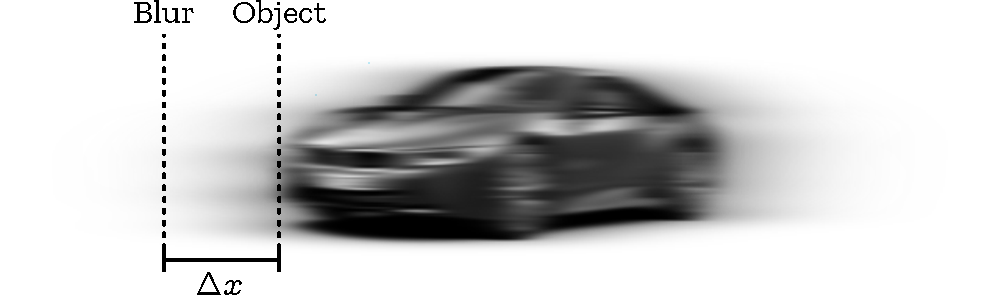
\includegraphics[width = \textwidth]{derivatives/motionblurredcar.pdf} 
   \caption{Calculating the velocity of a car from motion blur.}
   \label{fig:car-motion-blur}
\end{figure}

But what will happen with shorter exposure time? Does the motion blur disappear? No! The blur is still there, but it's just smaller. Typically, $\qty{12}{\ms}$ exposure time is short enough to create a ``focused image''. But it's just an illusion that came from the limitation of the screen's ability to reproduce such little blur. If our camera and screen is good enough, we can \emph{always} calculate the velocity of the car from the blur. The smaller the exposure time, the more detailed the image is, and the closer you'll get to the exact $\vv{v}$ at that moment in time. Finally, if we let the exposure time become infinitesimally short, we can say the $\vv{v}$ we got is \emph{the velocity at that exact point}. Or as we call it, the \textbf{instantaneous velocity}. By using the said calculus notation in \cref{sec:notation_of_calculus_derivative}, we can just write this as
\begin{equation}
    \vv{v} = \odv{\vv{x}}{t}, \label{eq:first_intro_to_derivative}
\end{equation}
and here it is ladies and gentlemen, the \textbf{derivative}: the measure of rate of change.

From here on out, I shall use \emph{derivative} and \emph{rate of change} interchangeably. So, every time you see \emph{derivative}, think \emph{rate of change}.

\section{An attempt to define derivatives}

Mathematically, a \textbf{derivative} is a measure of a function's rate of change with respect to a variable. In the previous example, $\vv{x}$ is a function that's dependent on time, and its derivative w.r.t. time, $\vv{v}$, is measuring the rate of change of function $\vv{x}(t)$ through time $\odif{t}$.

To find an explicit expression for derivative, let's say we have two points in spacetime $(\vv{x}_1, t_1)$ and $(\vv{x}_2, t_2)$. The change in $\vv{x}$ is $\vv{x}_2 - \vv{x}_1$, and the change in time is $t_2 - t_1$. The derivative of position w.r.t. time is then just
\begin{equation}
    \vv{v} = \odv{\vv{x}}{t} = \frac{\vv{x}_2 - \vv{x}_1}{t_2 - t_1}. \label{eq:derivative1}
\end{equation}
Let $t_2 = t + h$. Then, $\vv{x}_2 = \vv{x}(t + h)$ and $\vv{x}_1 = \vv{x}(t)$. The time difference used to calculate $\vv{v}$ must be miniscule: infinitesimally small. I have to introduce the notion of limits, which is just a fancier way of saying ``very close to, but not''
\begin{align}
    \vv{v} = \odv{\vv{x}}{t} &= \lim_{h \appr 0}\frac{\vv{x}(t + h) - \vv{x}(t)}{(t + h) - t} \\
							 &= \lim_{h \appr 0}\frac{\vv{x}(t + h) - \vv{x}(t)}{h}.
\end{align}
The equation above is what we generally refer to as the \emph{definition of derivative}. Then, we just extend this relation to any function $f(x)$, which requires just a substitution of variables. And then we get:
\begin{df}{Naive definition of derivative}{derivative_naive}
    \index{derivatives!naive definition}A derivative of a function $f(x)$ w.r.t. a variable $x$ is the rate of change of $f(x)$ w.r.t. $x$, and it is written as
    \begin{equation}
        \odv{f(x)}{x} \mathor \odv*{f(x)}{x},
    \end{equation}
    where
    \begin{equation}
        \odv{f(x)}{x} = \lim_{h \appr 0}\frac{f(x + h) - f(x)}{h}.\label{eq:naive_definition_of_derivative}
    \end{equation}
\end{df}
\Cref{eq:naive_definition_of_derivative} directly reads:
\begin{quote}
    The derivative of $f(x)$ with respect to $x$ is $\frac{f(x + h) - f(x)}{h}$ where $h$ is very close to $0$, but $h$ is strictly not $0$.
\end{quote}

\paragraph{On notation:} So far, we've been using the Leibniz's notation for derivatives, and it has the property that derivatives behave exactly like fractions, and you can cancel terms.
\begin{equation}
    \odv{a}{b}\times\odv{b}{c} = \odv{a}{c}.\label{eq:prechainrule}
\end{equation}
But, this isn't the only accepted notation. Multiple great mathematicians have come up with their own, and some are better than others in certain cases. I'd introduce other notations later on if necessary.

\section{The geometrical interpretation of the derivative}

One way to interpret derivatives is by using slope. Notice that \cref{eq:derivative1} looks a lot like the slope equation
\begin{equation}
    m = \frac{y_2 - y_1}{x_2 - x_1}. \label{eq:slope_equation}
\end{equation}
We've also seen that \cref{eq:derivative1} is analogous to the definition of derivative \cref{eq:naive_definition_of_derivative}. So is the derivative just the slope of a line? If it is, then what is the $y$-axis and the $x$-axis of a graph?

\begin{wrapfigure}[10]{l}{0.43\textwidth}
    % \centering
    % \begin{subfigure}{0.45\textwidth}
        \centering
        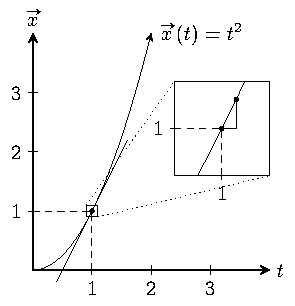
\includegraphics{derivatives/positionversustime}
        \caption{Position vs. time graph where $\protect\vv{x}(t) = t^2$.}
        \label{fig:position_versus_time}
    % \end{subfigure}
    % \begin{subfigure}{0.4\textwidth}
    %     \centering
    %     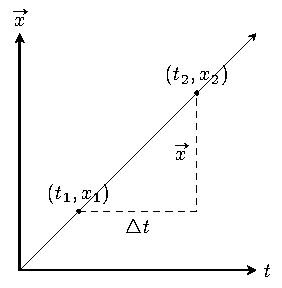
\includegraphics{derivatives/positionversustime2}
    %     \caption{A ball traveling at constant velocity.}
    %     \label{fig:position_versus_time2}
    % \end{subfigure}
    % \caption{Various position versus time graph.}
\end{wrapfigure}

We can compare \cref{eq:slope_equation} to \cref{eq:derivative1}: the $y$-axis should be the position $\vv{x}$, and the $x$-axis, the time $t$. If we draw that out, we'll get the $x$-$t$ graph, which can encode the exact trajectory of an object. An example of which is shown in \cref{fig:position_versus_time}.

But what does this have to do with derivatives? \Cref{eq:slope_equation} only works for straight line! Well, here's the beauty of it. If you zoom into any points on a curve, eventually, it will look like a line. And thus, \emph{the derivative zooms into the curve at some point, and chooses two very close points on the curve and calculate its slope. In which, that slope represents the rate of change of the function at that point.}

\section{Evaluation of derivatives: method of increments}

The derivative's definition can be used to directly evaluate derivatives. This is called the \textbf{method of increment}. E.g., in \cref{fig:position_versus_time}, let's evaluate the velocity at time $t = \qty{1}{\second}$ where the position function, $\vv{x}(t) = t^2$. $t = \qty{1}{\second}$. We start from \cref{eq:naive_definition_of_derivative}:
\begin{align*}
    \vv{v}(1) = \frac{\vv{x_2} - \vv{x_1}}{t_2 - t_1} &= \lim_{h \appr 0}\frac{\vv{x}(1 + h) - \vv{x}(1)}{(1 + h) - 1} \\
    &= \lim_{h \appr 0}\frac{(1 + h)^2 - 1}{h} \\
    &= \lim_{h \appr 0}\frac{2h + h^2}{h} \\
    &= \lim_{h \appr 0}2 + h.
\end{align*}

Since $h$ is very close to zero, we approximate $2 + h$ as $2$. Imagine comparing $2$ to $10^{-10}$. The $10^{-10}$ wouldn't make a noticeable difference, and we can ignore it. Therefore, $\vv{v}(t = \qty{1}{\second}) = \qty{2}{\meter\per\second}$.

Now, try evaluating $\vv{v}(t = \qty{3}{\second})$ for $\vv{x}(t) = t^3$. You should get $\qty{81}{\meter\per\second}$. As a hint, you can also ignore $h^2$ because if $h < 1$, then $h^2 < h$.

\section{Higher order derivatives}

\begin{wraptable}[13]{l}{0.36\textwidth}
    \begin{tabular}{c | c}
        Order & Name \\
        \hline
        1 & Velocity/Speed \\
        2 & Acceleration \\
        3 & Jerk \\
        4 & Snap/Jounce \\
        5 & Crackle \\
        6 & Pop
    \end{tabular}
    \caption{Higher order derivatives of position w.r.t. time}
    \label{tab:jerksnapcracklepop}
\end{wraptable}
\index{derivatives!higher order}
In kinematics, there are a whole set of quantities that can describe an object's trajectory, e.g., the acceleration, which is defined to be the rate of change of velocity w.r.t. time:
\begin{equation*}
    \vv{a}(t) = \odv{\vv{v}(t)}{t}.
\end{equation*}
But the $\vv{v}$ is also the rate of change of position w.r.t. time. Thus,
\begin{equation*}
    \vv{a}(t) = \odv{\vv{v}(t)}{t} = \odv*{\ab(\odv{\vv{r}(t)}{t})}{t} = \odv[ord = 2]{\vv{r}(t)}{t}, 
\end{equation*}
where $\vv{r}$ is any position vector.

The $\odif[ord = 2]{\vv{r}}$ and $\odif{t}^2$ is just a matter of symbolic manipulation and should only be interpreted as just a shorthand. $\vv{a}$ is called the \textbf{second order derivative} of $\vv{r}$ because you've differentiated $\vv{r}$ twice. \textbf{Higher order derivatives} of position w.r.t. time is listed in \cref{tab:jerksnapcracklepop}.

\section{Expressing nature: basic differential equations}
\label{sec:basicdifferentialequations}

The dynamics of a physical system is universally described by the famous Newton's second law $\vv{F} = m\vv{a}(t)$, which in derivatives form becomes:
\begin{equation}
    \vv{F} = m\odv[ord = 2]{\vv{r}(t)}{t}. \label{eq:newton_second_law}
\end{equation}
\begin{wrapfigure}[11]{r}{0.4\textwidth}
    \centering
    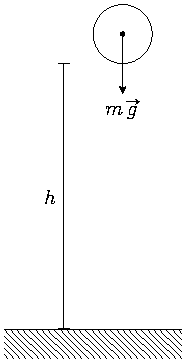
\includegraphics{derivatives/simplemotion}
    \caption{A ball dropped from height $h$}
    \label{fig:ball_dropped_from_a_height}
\end{wrapfigure}
Let's try to describe a simple system with this. In \cref{fig:ball_dropped_from_a_height}, a ball is dropped from height $h$. The Earth's gravity pulls the ball with force $mg$ where $m$ is the mass of the ball, and $\vv{g}$, the acceleration from Earth's gravity. Newton's second law tells us that
\begin{align}
    \vv{F} &= m\odv[ord = 2]{\vv{r}(t)}{t} \nonumber\\
    m\vv{g} = m\odv[ord = 2]{\vv{r}(t)}{t} &\quad \textrm{or,} \quad \vv{g} = \odv[ord = 2]{\vv{r}(t)}{t},
\end{align}
which is sometimes called the \textbf{equation of motion}, which packs every information about this system you'd ever want. It directly reads as:
\begin{quotation}
    The acceleration of the ball is equals to $g$.
\end{quotation}
If you've stayed for this long, congratulations! You now have the power to describe every physical systems with mathematical equations using derivatives: the measure of the rate of change. But it might not be as useful as yet, just as a hammer may seem useless if used to paint, derivatives falls apart when you ask about the future of the system. E.g., how long the ball takes to reach the ground? Or, what's the position of the ball at a certain time? That's the job of the integral to solve, and we'll do so in the next chapter.

\conclusion

\begin{enumerate}[noitemsep]
    \item The concept of approaching can be used to bypass dividing by zero.
    \item Derivatives are rate of change of a function w.r.t. a variable which can be evaluated by the method of increments.
    \item Derivatives can be thought as the slope of a graph, or the tangent to a curve.
    \item Physical systems can be described by differential equations of different forms. One of them is the Newton's formulation stated in \cref{eq:newton_second_law}
\end{enumerate}

\begin{remark}{}{derivatives}
    \begin{enumerate}
        \item In \cref{sec:speedandinstantaneousrateofchange}, we zoomed in on the graph to approximate the function as a line. Actually, this is quite literally the whole idea of derivatives. If we dig in further in calculus, sometimes the rate of change analogy doesn't even make sense. However, saying that the derivative tries to approximate every function as a line works in all scenario. Though, it's quite abstracted away from the world.
    \end{enumerate}
\end{remark}

\chapter{Integrals and antiderivative}
\label{sec:integrals}

\prerequisites{\cref{sec:derivatives}, sigma summation notation}

Before we dive in, I shall clarify that every line, including straight, is a mathematical \index{curve}\textbf{curve}. You might see other textbooks use the term ``\textit{area under the graph}'' to refer to integrals. But, a \index{graph}\textbf{graph} is \textit{a diagram consisting of a line or lines, showing how two or more sets of numbers are related to each other} \cite{oxforddict}, not the curve itself. Therefore, I'll refer to a curve as any line that connects two points, whether straight or not. Now let's start.

\section{Invitation: mission impossible}

\subsection{The mindset of integral calculus}

In the previous chapter, we've learned how to describe the universe using derivatives. But derivatives falls short when we want to predict the future of a system. But, what do we mean when we say ``predict the system?''

In classical physics, a \textbf{state} represents the configuration that the system \emph{at one point in time}. To predict the system, we need to know the initial state of a system. Classical physics says that if you know the rules that the system plays by (In this case, $\vv{F} = m\dv[2]{\vv{r}}{t}$), and the initial condition, we can always determine the state of the system at any point in time. That is, classical physics guarantees that there is always a function, which takes in time as input, and outputs the state of a system. And in order to predict the system, we must know that function. But what may that function be?

Consider the example from \cref{sec:derivatives}. The equation of motion of the ball dropped from a height $h$ is a second-order differential equation
\begin{equation}
    g = \dv[2]{\vv{r}(t)}{t}, \label{eq:acceleration_from_gravity}
\end{equation}
with initial condition being $\vv{r} = h$. The function that describes the state is $\vv{r}(t)$, which outputs the position of the ball at a certain time $t$. You can see that this function is the derivative sign. To solve the differential equation for this function, we have to isolate it out, and undo the derivative sign. But how?

It seems impossible at first. We only know that $\vv{r}(t)$ must satisfy \cref{eq:acceleration_from_gravity}, i.e., the second derivative of $\vv{r}(t)$ is $g$. It's like we have to search through a gigantic pool of functions that mathematics have to offer to find a single function $\vv{r}(t)$ that satisfies \cref{eq:acceleration_from_gravity}. It'd be like finding a needle in the haystack!

Of course, this is a textbook, there must be a solution. If there is a will, there is a way. You might have to reverse engineer derivatives, which might look tedious at first. But well, you might find something interesting along the way.

\subsection{Brief notation of integral calculus}
\label{sec:brief_notation_of_calculus_integral}

The $\displaystyle\int$, a.k.a. the \textbf{integral}\footnote{Which also looks like a beansprout}, means to sum. This integral symbol is basically sigma summation symbol, but for infinitesimals. Therefore, we have bounds called \textbf{integral bounds}. E.g., if we sum a lot of little time step $\dd{t}$ together from $t_A$ to $t_B$ we get $t_B - t_A$, the total time step. Thus,
\begin{equation}
    \int_{t_A}^{t_B}\dd{t} = t_B - t_A.
\end{equation}

\section{Finding a function in the haystack}
\label{sec:function_in_the_haystack}

\Cref{eq:acceleration_from_gravity} has a second order derivative, let's go slowly and undo one derivative at a time. We'll undo the derivative of the RHS to get the velocity first. Then, we'll undo the derivative again to get the position.

\subsection{Step one: the velocity function from acceleration}

In \cref{eq:acceleration_from_gravity}, both $\vv{r}$ and $t$ is mixed up on the same side of the equation. That's not good for solving equations. So let's separate them. First, write $\dv[2]{\vv{r}(t)}{t}$ as $\dv{\vv{v}(t)}{t}$. Then, isolate $\vv{v}$ on one side and move $\vv{t}$ to the other.
\begin{align}
    \vv{g} &= \dv{\vv{v}(t)}{t} \\
    \dd{\vv{v}}(t) &= g\dd{t}.
\end{align}
This equation reads
\begin{quotation}
    \emph{A small change in velocity $\dd{\vv{v}}$ is product of $\vv{g}$ and a small time interval $\dd{t}$.}
\end{quotation}

\begin{multicols}{2}
To find the total change in velocity, we sum up a lot of small changes in velocity $\dd{\vv{v}}(t)$, which is equal to $\vv{g}\dd{t}$. Because $\dd{v}$ is directly proportional to $\dd{t}$, the total change in $\vv{v}$ is simply $\vv{g}t$. However, \emph{changes} doesn't say anything about the initial condition, so we add a term $C$ to compensate. Therefore,
\begin{equation}
    \vv{v}(t) = \vv{g}t + C.
\end{equation}
To find what $C$ is, just plug in the initial condition. If $\vv{v}(t = 0) = \vv{v}_0$, then
\begin{align}
    \vv{v}(t = 0) = v_0 &= \vv{g}\times 0 + C \\
    v_0 &= C.
\end{align}
Thus,
\begin{equation}
    \vv{v}(t) = \vv{g}t + \vv{v}_0.
\end{equation}
We can also express these ideas symbolically using the integral symbol (\cref{sec:brief_notation_of_calculus_integral}) as
\begin{align}
    \vv{g} &= \dv{\vv{v}(t)}{t} \\
    \dd{\vv{v}} &= \vv{g}\dd{t} \\
    \int\dd{\vv{v}} &= \int \vv{g}\dd{t} \\
    \vv{v} &= \vv{g}t + \vv{v}_0. \label{eq:simplemotionr}
\end{align}
\end{multicols}

\subsection{Step two: the position function from velocity}
Rewrite $\vv{v}$ as $\dv{\vv{r}}{t}$, then do separation of variables.
\begin{align}
    \vv{v} = \dv{\vv{r}}{t} &= \vv{g}t + \vv{v}_0 \label{eq:simplemotionr2} \\
    \dd{\vv{r}} &= \dd{t}(\vv{g}t + \vv{v}_0),\label{eq:simplemotionr3}
\end{align}
which reads,
\begin{quotation}
    \emph{A small change in position $\dd{\vv{r}}$ is the product of $\vv{g}t + \vv{v}_0$ and a small time interval $\dd{t}$.}
    \label{quote}
\end{quotation}
If we want to find the total change in position $\vv{r}$, we just have to sum all $\dd{\vv{r}}$'s. This time, it's not as obvious, because there's $\vv{g}t + \vv{v}_0$, which is also changing with time. So at each point in time, the rate of change of position is different.

\begin{figure}[ht]
    \centering
    \begin{subfigure}[b]{0.45\textwidth}
        \centering
        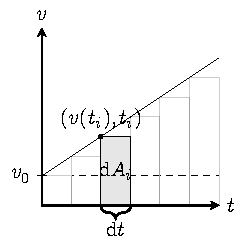
\includegraphics{integrals/simplemotionsubdivide}
        \caption{A subdivided graph}
        \label{fig:simplemotionsubdivided}
    \end{subfigure}
    \begin{subfigure}[b]{0.45\textwidth}
        \centering
        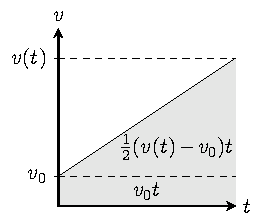
\includegraphics{integrals/simplemotionr}
        \caption{A graph showing the area of the gray trapezoid broken into two parts}
        \label{fig:simplemotionr}
    \end{subfigure}
    \caption{A $v$-$t$ graph of a ball dropped from a building}
\end{figure}

\begin{multicols}{2}
A good strategy in math if you don't know what to do is to just graph the function. The graph of \cref{eq:simplemotionr2} is shown in \cref{fig:simplemotionsubdivided}. A small time interval represents a little step in the $t$ axis. The curve shown in the graph represents $\vv{g}t + \vv{v}_0$. Therefore, $\dd{t}(\vv{g}t + \vv{v}_0)$ would just represent an area of a little rectangle $\dd{A}$ as shown in the figure.

The total change in position is the sum all those rectangles. When $\dd{t} \appr 0$, the sum of all $\dd{t}(\vv{g}t + \vv{v}_0)$ approaches the area under the graph, which can be calculated geometrically as shown in \cref{fig:simplemotionr}. Thus,
\begin{align}
    \vv{r} &= \frac{1}{2}(\vv{v}(t) - \vv{t}_0)t + \vv{v}_0t + C \\
    &= \frac{1}{2}(\vv{g}t - \vv{t}_0)t + \vv{v}_0t + C \\
    &= \frac{1}{2}\vv{g}\times t^2 + \vv{v}_0t + C
\end{align}
When $t = 0$, $\vv{r} = \vv{r}_0$. Therefore,
\begin{align*}
    \vv{r}_0 &= \frac{1}{2}\vv{g}\times 0^2 + \vv{v}_0\times 0 + C \\
    \vv{r}_0 &= C.
\end{align*}
Therefore,
\begin{equation}
    \vv{r}(t) = \frac{1}{2}\vv{g}t^2 + \vv{v}_0t + \vv{r}_0.
\end{equation}

To model the trajectory of the ball, we set
\begin{enumerate}[noitemsep]
    \item $\vv{v}_0 = 0$ (object is dropped and starts at zero speed)
    \item $\vv{r}_0 = 0$ (convenient initial condition placement)
\end{enumerate}
thus we get,
\begin{gather}
    \vv{r} = \frac{1}{2}\vv{g}t^2 \implies t = \sqrt{\frac{2\vv{r}}{\vv{g}}}
\end{gather}
\end{multicols}
Since the ground is at $\vv{r} = h$, the time that the ball hits the ground is then $\sqrt{2h/\vv{g}}$.

\subsection{Conclusion: area under the curve and antiderivative}

The form of the differential equation that we've solved is in the form $\dv{x}{t} = f(x)$. We have to undo the derivative, and the simplest way is to do separation of variables and turn the equation into
\begin{equation}
    \dd{x} = f(x)\dd{t},
\end{equation}
which reads,
\begin{quotation}
    A small change in $x$, i.e., $\dd{x}$ is represented by the area of a rectangle width $\dd{t}$ and height $f(x)$.
\end{quotation}
And, the total change $x$ is represented by the sum all those little rectangles, which is the area under the curve $f(x)$. Then, we add a constant $C$ to compensate for the initial condition. In symbolic form introduced in \cref{sec:brief_notation_of_calculus_integral}, it's just
\begin{align}
    \int\dd{x} &= \int g(x)\dd{t} \\
    x &= \int g(x)\dd{t}.
\end{align}

For now, we could say that integration is the reverse of derivatives. But to clearly see how this is linked for every function, we must study the fundamental theorem of calculus, which is the bridge between integration and differentiation.

Before we go there, let me clarify some terminologies. An \textbf{integral} refers to the area under the curve evaluated between two points. We say that an integral must have an \textbf{integral bound}. If we want to find the area under a function $f(x)$ from $x = a$ to $x = b$, we write it as
\begin{equation}
    A = \int_a^b f(x)\dd{x}.
\end{equation}
This just reads
\begin{quotation}
    The area $A$ under the curve $f(x)$ from $x = a$ to $x = b$ is equal to the sum of the area of many thin stripes width $\dd{x}$ height $f(x)$ that lies between $x = a$ and $x = b$.
\end{quotation}
The \textbf{antiderivative} however, refers to the function which takes in a value $a$, and output the integral of $f(x)$, evaluated from $0$ to $a$. Therefore, if $A(a)$ is the antiderivative of $f(x)$, then
\begin{equation}
    A(a) = \int_0^a f(x)\dd{x}.
\end{equation}
It also implies that if the area between $a$ and $b$ can be evaluated by
\begin{equation}
    \int_a^b f(x)\dd{x} = A(b) - A(a).
\end{equation}

\section{The fundamental theorem of calculus}
\label{sec:fundamentalthmofcalc}

\index{The fundamental theorem of calculus!first part}The intuition of fundamental theorem of calculus states that derivatives and integrals are essentially inverse of each other. In this section, I'll clarify this fact and make it more rigorous.
\begin{thm}{The (first) fundamental theorem of calculus}{fundamentalthmofcalc1}
    If a function $f(x)$ has an antiderivative $A(x)$, then
    \begin{equation}
        \dv{A(x)}{x} = f(x).
    \end{equation}
\end{thm}

\begin{figure}[b]
    \centering
    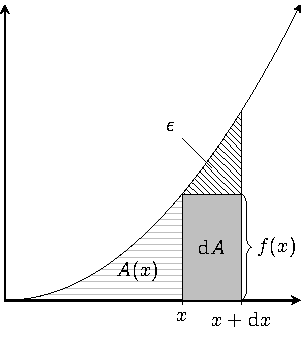
\includegraphics{integrals/fundamentalthmofcalc}
    \caption{The geometrical interpretation of part one of the fundamental theorem of calculus (\cref{thm:fundamentalthmofcalc1}).}
    \label{fig:fundamentalthmofcalc}
\end{figure}
If $A(x)$ is the antiderivative of $f(x)$, then
\begin{equation}
    \int_{0}^{x} f(x)\dd{x} = A(x).
\end{equation}
The \emph{actual} area of one of the stripes (not rectangles) width $\dd{x}$ shown in \cref{fig:fundamentalthmofcalc}, it's obviously $A(x + \dd{x}) - A(x)$. The riemann sum approximation approximates the area by a small rectangle area $f(x)\dd{x}$. We can write the relation between the actual and the approximated area as
\begin{equation}
    A(x + \dd{x}) - A(x) \approx f(x)\dd{x}.
\end{equation}
To turn this into an equality, we add a correction term $\epsilon$
\begin{equation}
    A(x + \dd{x}) - A(x) = f(x)\dd{x} + \epsilon.
\end{equation}
If we let $\dd{x} \appr 0$, $\epsilon$ is negligible compared to $f(x)\dd{x}$; therefore,
\begin{equation}
    \lim_{\dd{x} \appr 0}A(x + \dd{x}) - A(x) = \lim_{\dd{x} \appr 0}f(x)\dd{x}.
\end{equation}
Since $f(x)$ is not a variable that's controlled by the limit sign,
\begin{align*}
    \lim_{\dd{x} \appr 0}A(x + \dd{x}) - A(x) &= f(x)\lim_{\dd{x} \appr 0}\dd{x} \\
    \lim_{\dd{x} \appr 0}\frac{A(x + \dd{x}) - A(x)}{\dd{x}} &= f(x).
\end{align*}
And here, we see that the L.H.S. is just the derivative of $A(x)$ w.r.t. $x$, thus
\begin{equation}
    \dv{A(x)}{x} = f(x),
\end{equation}
or ``\textit{the rate of change in area is the function itself}''. But the area function is given by the integral. This means
\begin{equation}
    \dv{x}\int f(x)\dd{x} = f(x):
\end{equation}
integrals and derivatives are inverses of each other. If we rephrase \cref{thm:fundamentalthmofcalc1}, we see that ``\textit{the integral is the cumulative effect of the function}.''

\index{The fundamental theorem of calculus!second part}The second fundamental theorem of calculus,
\begin{thm}{The second fundamental theorem of calculus (Newton-Leibniz rule)}{fundamentalthmofcalc2}
    If a function $f(x)$ has an antiderivative $A(x)$, then its indefinite integral from $a$ to $b$ is
    \begin{equation}
        \int_{a}^{b}f(x)\dd{x} = \int_{0}^{b}f(x)\dd{x} - \int_{0}^{a}f(x)\dd{x} = A(b) - A(a).
    \end{equation}
\end{thm}
follows as a direct consequence of the geometrical interpretation of integrals: area under the curve.

The fundamental theorem of calculus allows us to evaluate integrals using derivatives. For example, if the derivative of $x^2$ is $2x$, then we also know that the integral of $2x\dd{x}$ is just $x^2$, which we'll discuss how to do that in the next chapter.

\section{How to calculate an integral? Riemann sum}
\label{sec:riemann_sum}

\begin{figure}[b]
    \centering
    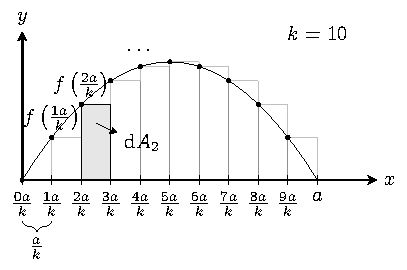
\includegraphics{integrals/integralex}
    \caption{Illustration of Riemann sum of a function $f(x)$ from $0$ to $a$ by setting $k = 10$}
    \label{fig:integralex1}
\end{figure}

In \cref{sec:function_in_the_haystack}, we used geometry to find the area under a curve. However, that is not always possible, e.g., try integrating \cref{fig:integralex1} geometrically\footnote{This is what you'd get if you solve the simple harmonic oscillator}. It'd be impossible. But we can still approximate its area by slicing the area under the curve into thin rectangular stripes, then summing them. The approximated area is called the \index{Riemann sum}\textbf{Riemann sum}. Due to its computational cost, you don't really want to use this method. However, to develop a good intuition at the integral, we should still know its symbolic form.

Let there be a function $A(s)$ that represents the actual area of a function $f(x)$ from $0$ to $s$. The approximated area is then
\begin{equation}
    \sum_{i = 0}^{k}\dd{A_i} = \sum_{i = 0}^{k}\mathrm{width} \times \mathrm{height}
\end{equation}
where $k$ is the amount of subdivisions. From \cref{fig:integralex1}, the width of each stripe is $\flatfrac{a}{k}$, and the height of the $i$'th stripe is $f(\flatfrac{ia}{k})$. Therefore,
\begin{equation*}
    \sum_{i = 0}^{k}\frac{a}{k}\times f\left(\frac{ia}{k}\right).
\end{equation*}

In \cref{fig:integralex1}, we  $k = 10$. The area of the second rectangle $\dd{A_2}$ is
\begin{equation*}
    \dd{A_2} = \frac{a}{k}f\left(\frac{2a}{k}\right).    
\end{equation*}

For an arbitrarily finite $k$, the Riemann sum is just an approximation. If you want to find the \textit{actual} area under the curve, let $k \appr \infty$. The limit as $k \appr \infty$ is what we actually call the \textbf{integral}. Thus, we say
\begin{df}{Naive definition of integrals}{integralsnaivedefinition}
    The \index{integrals!definite integrals}(definite) integral, or the area under the curve of $f(x) = y$ from $0$ to $a$, is defined as
    \begin{equation}
        \int_{0}^{a}\dd{A} = \int_{0}^{a}f(x)\dd{x} = \lim_{k \appr \infty}\sum_{i = 0}^{k}\frac{a}{k} \times f\left(\frac{ia}{k}\right) = A(a).
    \end{equation}
    where $\int$ is the integral sign\footnote{Famously known for looking like a beansprout}. Here, $0$ is the lower bound of integration, and $a$, the higher bound. The function $A(x)$ is called the \textbf{antiderivative}, or the \index{integrals!indefinite integrals}\textbf{indefinite integral} of $f(x)$.
\end{df}

I shall put these definitions into perspective in the next two examples. It might use a bit of series knowledge. If you don't know, you can simply search up the summation identities that I'll use in \emph{Wikipedia} \cite{wikipedia-summation}.

\begin{exmp}{Riemann sum and antiderivative of $x^2$}{}
    Let $f(x) = x^2$, and let $A(a)$ be the antiderivative of $f(x)$, i.e., $A(a)$ is the area under the curve of $f(x)$ from $0$ to $a$. Note that
    \begin{equation}
        \sum_{i = 0}^{k}i^2 = \frac{k(k + 1)(2k + 1)}{6},
    \end{equation}
    The Riemann sum is then
    \begin{align}
        \sum_{i = 0}^{k}\frac{a}{k}&\times f\left( i a \over k \right) = \sum_{i = 0}^k\frac{a}{k}\times \left(ia\over k\right)^2 \\
        &= \sum_{i = 0}^k\frac{a^3}{k^3}\times i^2 \\
        &= \frac{a^3}{k^3}\times \frac{k(k + 1)(2k + 1)}{6}.
    \end{align}
    To find the antiderivative, let $k \appr \infty$. Notice that the $+1$ in the parenthesis are negligible when $k \appr \infty$. Therefore, we can write the antiderivative as
    \begin{align}
        A(a) &= \int_0^a f(x)\dd{x} \\
        &= \lim_{k \appr \infty}\frac{a^3}{k^3}\times \frac{k(k + 1)(2k + 1)}{6} \\
        &= \lim_{k \appr \infty}\frac{a^3}{k^3}\times \frac{2k^3}{6} \\
        &= \lim_{k \appr \infty}\frac{x^3}{3} = \frac{x^3}{3}.
    \end{align}
\end{exmp}

\begin{exmp}{Riemann sum and antiderivative of $x^3$}{}
    Let $f(x) = 4x^3$, and let $A(a)$ be the antiderivative of $f(x)$, i.e., $A(a)$ is the area under the curve of $f(x)$ from $0$ to $a$. Note that
    \begin{equation}
        \sum_{i = 0}^{k}i^3 = \left(\frac{k(k + 1)}{2}\right)^2,
    \end{equation}
    The Riemann sum is then
    \begin{align*}
        \sum_{i = 0}^{k}\frac{a}{k}&\times f\left( i a \over k \right) = \sum_{i = 0}^k\frac{a}{k}\times 4\left(ia\over k\right)^3 \\
        &= 4\sum_{i = 0}^k \left(\frac{x}{k}\right)^4 i^3 \\
        &= 4\left(\frac{x}{k}\right)^4\left(k(k+1)\over 2\right)^2.
    \end{align*}
    To find the antiderivative, let $k \appr \infty$. The $+1$ in $(k + 1)$ can be ignored as $k \appr \infty$. Therefore,
    \begin{align*}
        A(a) &= \int_0^a f(x)\dd{x} \\
        &= \lim_{k\appr\infty}4\left(x\over k\right)^4\left(k^2\over 2\right)^2 \\
        &= \lim_{k\appr\infty}x^4 = x^4.
    \end{align*}
\end{exmp}

\section{Basic applications of the integrals}

\subsection{Five equations of linear motion}
\label{sec:fiveequationsoflinearmotion}

\index{equation of motion!uniformed acceleration}So far, we have developed an intuition for derivatives, integrals, and their relationship. Let's apply those concepts to derive the famous equations of linear motion:
\begin{gather}
    v(t) = v_0 + at, \label{eq:linearmotion1}\\
    s = \frac{1}{2}(v_0 + v(t))t, \label{eq:linearmotion2}\\
    s = v_0(t)t + \frac{1}{2}at^2, \label{eq:linearmotion3}\\
    s = v(t)t - \frac{1}{2}at^2,\label{eq:linearmotion4}\\
    v(t)^2 = v_0^2 + 2as. \label{eq:linearmotion5}
\end{gather}

\begin{figure}[b]
    \centering
    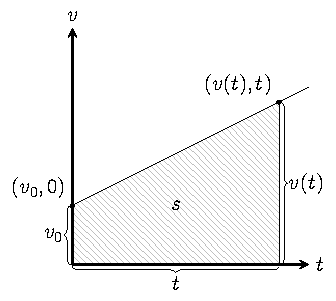
\includegraphics{integrals/constantacceleration}
    \caption{$v$-$t$ graph of an object under constant or uniformed acceleration}
    \label{fig:vtconstantacceleration}
\end{figure}
Here, $v_0$ represents the initial velocity, $v(t)$, the velocity at any time $t$, $a$, the acceleration, and $s$, the displacement. These equations are derived from the Newton's second law on \emph{constant/uniformed acceleration} motion in one dimension, which we can evaluate using the geometrical interpretation of integrals developed earlier.

Because we've constrained the object to move at acceleration $a$, the force exerted must be $ma$. Newton's second law $F = m\dv[2]{x}{t}$ then simplifies to
\begin{equation*}
    a = \dv[2]{x}{t}.
\end{equation*}
The same idea applies, we rewrite the equation in terms of $v$.
\begin{equation}
    a = \dv{v}{t} \label{eq:linearmotionintermediate}
\end{equation}
Which reads, ``\emph{the rate of change of $v$ w.r.t. $t$ is $a$}'' or ``\emph{the slope of the $v$-$t$ curve is always equals to $a$}''. Because $a$ is constant, the $v$-$t$ curve must be a straight line with slope $a$, shown in \cref{fig:vtconstantacceleration}.

\begin{multicols}{2}
\begin{proof}[Derivation of \cref{eq:linearmotion1}]
    We take advantage of the linearness of the curve. Just pick two points on \cref{fig:vtconstantacceleration}, as already shown, then
    \begin{align*}
        m = a &= \frac{\Delta v}{\Delta t} = \frac{v(t) - v_0}{t - 0} \\
        a & = \frac{v(t) - v_0}{t} \\
        v(t) &= v_0 + at.\qedhere
    \end{align*}
\end{proof}

\begin{proof}[Derivation of \cref{eq:linearmotion2}] 
    Use the reverse of \cref{thm:fundamentalthmofcalc1}. We know that\footnote{Here, $x$ is replaced with $s$ to represent displacement in one dimension.} $v = \dv*{s}{t}$; therefore,
    \begin{equation*}
        \int v\dd{t} = s,
    \end{equation*}
    which reads ``\emph{The displacement $s$ is the area under the curve of a $v$-$t$ graph}''. From \cref{fig:vtconstantacceleration}, the area under the curve is a trapezoid with side length $v_0$, $v(t)$, and width $t$. Thus,
    \begin{equation*}
        s = \frac{1}{2}(v_0 + v(t))t,
    \end{equation*}
    which is just \cref{eq:linearmotion2}: the area of a trapezoid.
\end{proof}

\begin{proof}[Derivation of \cref{eq:linearmotion3,eq:linearmotion4,eq:linearmotion5}]
    We can arrange \cref{eq:linearmotion1} into three different ways, then plug in \cref{eq:linearmotion2}.
    First, $v(t) = v_0 + at$
    \begin{align*}
        s &= \frac{1}{2}(v_0 + v_0 + at)t \\
        &= v_0t + \frac{1}{2}at^2. 
    \end{align*}
    Second, $v_0 = v(t) - at$
    \begin{align*}
        s &= \frac{1}{2}(v(t) - at + v(t))t \\
        &= v(t)t - \frac{1}{2}at^2. 
    \end{align*}
    Third, $\displaystyle{t = \frac{v(t) - v_0}{a}}$
    \begin{align*}
        s &= \frac{1}{2}(v(t) + v_0)\frac{(v(t) - v_0)}{a} \\
        2as &= (v(t) + v_0)(v(t) - v_0) \\
        2as &= v(t)^2 - v_0^2 \\
        v(t)^2 &= 2as + v_0^2. \qedhere
    \end{align*}
\end{proof}
\end{multicols}

\subsection{The area of a circle}
\begin{figure}[b]
    \centering
    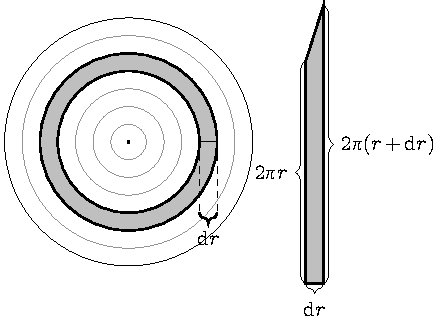
\includegraphics{integrals/dissectingcircle}
    \caption{(Left) Dissecting a circle radius $R$ radially into rings, each ring $\dd{r}$ thin. (Right) Stretching a ring into a trapezoid (Not to scale).}
    \label{fig:dissectingcircle}
\end{figure}

The perimeter of the circle is $2\cpi r$. For now, we only know how to find areas of polygons, but we want to know the circle's area. So, is there any way to turn a circle into a polygon? From \cref{sec:riemann_sum}, that the riemann sum can approximate areas under the curve using rectangular stripes. It'd be great if this circle can be turned into multiple rectangular stripes on a graph right?

\begin{wrapfigure}[]{r}{0.4\textwidth}
    \centering
    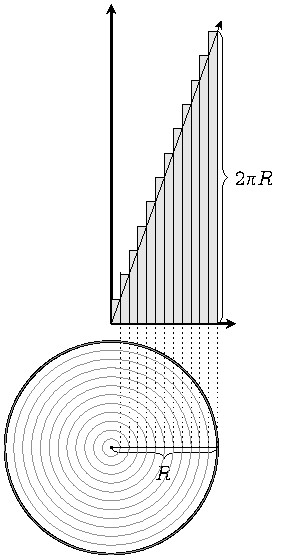
\includegraphics{integrals/dissectingcircle2}
    \caption{Rearranging all the approximated rectangles onto a graph (Not to scale).}
    \label{fig:dissectingcircle2}
\end{wrapfigure}

So, we dissect a circle radially into small rings $\dd{r}$ thin, as shown in \cref{fig:dissectingcircle}. Then, stretch all the rings into a very thin trapezoid-like shape. It might seem impossible at first, but considering that our ring is very thin, it's quite easy to stretch it without breaking. I encourage you to grab a piece of paper, cut a really thin ring and try it out. If you actually do it, it'll look a bit warped. However, the warpedness will go away the thinner you go.

Since we sliced our trapezoid from a circle, for a stripe positioned at $r$, the inner side will be $2\cpi r$ long and the outer side, $2\cpi (r + dr)$. The area of the little trapezoid $\dd{A}$ then becomes
\begin{align*}
    \dd{A} &= \frac{1}{2}\dd{r}(2\cpi r + 2\cpi (r + dr)) \\
    &= 2\cpi r\dd{r} + 2\cpi\dd{r}^2. 
\end{align*}
As $\dd{r} \appr 0$, $\dd{r}^2$ becomes negligible. Therefore,
\begin{equation}
    \dd{A} = 2\cpi r \dd{r}.
\end{equation}
This equation says that for $\dd{r} \appr 0$, the trapezoid becomes a rectangle side length $\dd{r}$ and $2\cpi r$. Now, we have to sum it together. If we can put all these rectangles onto a graph, we can easily use the Riemann's sum to evaluate it. A natural way to do this is to put all the rectangles that we got from stretching the rings of the circle onto a graph one by one. The result would look something like \cref{fig:dissectingcircle2}\footnote{Not to scale}.

For every stripe at $r$, its height is $2\pi r$. If you were to plot the height of all rectangles when $\dd{r} \appr 0$, it'll eventually look like a curve that's given by $f(r) = 2\pi r$. We're interested in the area of the circle from $0$ to $R$. Now, it's transformed into the area under the curve of $f(r) = 2\pi r$: a triangle with base $R$ and height $f(R) = 2\pi R$. Thus, the area of a circle becomes
\begin{equation*}
    A = \frac{1}{2}R(2\pi R) = \pi R^2.
\end{equation*}

And there you go, you've turned essentially turned circle into a triangle and evaluate its area from there. I'd like to end off this chapter by mentioning the spirit of mathematics. Sometimes, you can't solve the problem directly. Most of the time, you have to re-frame the problem into another more-solvable problem. Problems like these often have the most sublime connections to the foundations of mathematics. This is a common theme in most of mathematics, especailly calculus. So, be sure to keep this in mind while reading through.

\conclusion

\begin{enumerate}
    \item Riemann sum are used to approximate areas under the curve of a function by using little rectangles then summing it.
    \item Integrals or anti-derivatives are functions that output the area under the graph of other functions.
    \item The limit where the width of the rectangles in the Riemann sum approaches zero, the Riemann sum becomes an integral.
    \item Integrals are the cumulative effect of a function.
    \item Integrals and derivatives are inverses of each other, and they're related by the fundamental theorem of calculus
    \item Integrals can be used in various ways by reframing questions into another simpler question.
\end{enumerate}
\chapter{Basic derivatives and antiderivatives}
\label{sec:basic_derivatives_and_integrals}

This chapter covers the derivatives and integrals of common functions: polynomials, exponential, and logarithms; focusing on their geometrical interpretation.

\prerequisites{binomial theorem (\cref{appendix:binomialexpansion}), basic trigonometry, derivatives, and integrals}

\paragraph{Terminologies:} The integral refers to the area under the curve. The antiderivative refers to the function $A(x')$ that outputs the area under the curve from $0$ to $x'$.

\section{Basic rules}
\label{sec:trivial_rules}

\index{derivatives!chain rule}
\paragraph{The chain rule} The Leibniz' notation treats derivative as fractions; thus, we can cancel terms (\cref{eq:prechainrule}). We exploit this property to find derivatives of composite functions. Consider two functions $f(x)$ and $g(x)$, the derivative of $f(g(x))$ can be found by a simple substitution. First let $g(x) = u$.
\begin{equation*}
	\odv*{f(g(x))}{x} = \odv{f(u)}{x}.
\end{equation*}
Let $1 = \odv{u}{u}$, then
\begin{equation*}
	\odv*{f(u)}{x} = \odv*{f(u)}{x} \times 1 = \odv{f(u)}{x} \odv{u}{u}.
\end{equation*}
Perform a change of denominator, then substitute back $u = g(x)$:
\begin{equation*}
	\odv*{f(g(x))}{x} = \odv{f(u)}{u} \times \odv{g(x)}{x}.
\end{equation*}
This is what we call the chain rule, or more generally
\begin{equation}
    \odv{y}{x} = \odv{y}{u} \times \odv{u}{x}. \label{eq:chainrule}
\end{equation}
where $u$ is a function of $y$.

The chain rule holds the intuition of how rate of changes relate to each other. E.g., the cheetah's speed is $10$ times the bicycle's speed, which is $4$ times the walking speed. The ratio between the cheetah's speed compared to walking speed would obviously be $10\cdot 4 = 40$:
\begin{equation}
    \odv{\textrm{Cheetah}}{\textrm{Walking}} = \odv{\textrm{Cheetah}}{\textrm{Bicycle}} \times \odv{\textrm{Bicycle}}{\textrm{Walking}}.
\end{equation}

\index{integral constant}
\paragraph{Integral constant} In \cref{sec:function_in_the_haystack}, each time we evaluate the antiderivative, we add an initial condition term, i.e., $v_0$ and $r_0$. So for any function $f(x)$,
\begin{equation}
    \int f(x)\odif{x} = A(x) + C
\end{equation}
where $C$ is any constant. However, \cref{theorem:fundamentalthmofcalc2} still holds for integrals with bounds.
\begin{center}
	\textbf{
		\large Always add an integral constant after evaluating the antiderivative
	}
\end{center}

\index{integrals!of an infinitesimal}
\paragraph{Integral of the infinitesimal} The antiderivative of the small rectangles $\odif{x}$ is just the total rectangle $x$ plus the integral constant $C$. 
\begin{equation}
    \int \odif{x} = x + C.
\end{equation}

\paragraph{Rules of equality} If two arguments are equal, their derivatives and antiderivatives w.r.t. the same variable must also be equal.
\begin{equation*}
    \textrm{If}~f = g,\textrm{ then }\odv{f}{x} = \odv{g}{x},\textrm{ and }\int f\odif{x} = \int g\odif{x} + C
\end{equation*}

\index{derivatives!of a constant}\paragraph{Derivative of a constant} A constant doesn't change; thus, the derivative of a constant is zero. 
\begin{equation}
    \odv*{(c)}{x} = 0.
\end{equation}

\section{Linearity of differentiation and integration}
\label{sec:diff_int_linearity}

\begin{figure}[ht]
    \centering
    \begin{subfigure}[t]{0.75\textwidth}
        \centering
        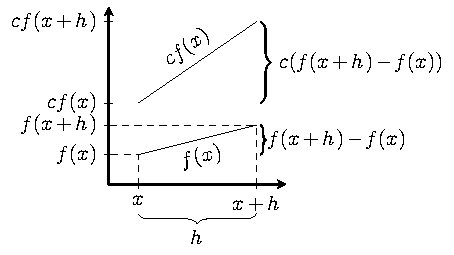
\includegraphics{basicderivativesandintegrals/derivativeconstantmultiple}
        \caption{for derivatives}
        \label{fig:derivativesconstantmultiple}
    \end{subfigure}
    \begin{subfigure}[b]{0.36\textwidth}
        \centering
        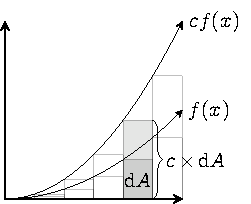
\includegraphics{basicderivativesandintegrals/integralconstantmultiple}
        \caption{for integrals}
        \label{fig:integralsconstantmultiple}
    \end{subfigure}
    \caption{Constant multiple rules}
\end{figure}

A \textbf{linear} mathematical entity are defined as anything that is compatible with addition and scaling. E.g., for a function $f(x)$ to be linear, it must obey
\begin{enumerate}[noitemsep]
    \item Additivity: $f(x + y) = f(x) + f(y)$
    \item Homogeneity of degree one: $f(ax) = af(x)$ for all constant $a$
\end{enumerate}
The simplest linear function there is, is a line that passes through the origin: $f(x) = ax$, in which
\begin{gather}
    f(x + y) = a(x + y) = ax + ay = f(x) + f(y), \\
    f(cx) = a(cx) = c(ax) = cf(x).
\end{gather}
Because this property, we associate a line with being linear. However, linearity doesn't have to always refer to lines.

Both derivatives and integrals are linear; for any function $f(x)$, $g(x)$, and constants $a$, $b$, the following rules follow.
\index{derivatives!constant multiple rule}\index{integrals!constant multiple rule}\paragraph{The constant multiple rule:}
\begin{align}
    \odv*{(af(x))}{x} &= a\odv{f(x)}{x}, &\alc[0.3]{Illustrated in \cref{fig:derivativesconstantmultiple}}\label{eq:derivativesconstantmultiple} \\
    \int af(x)\odif{x} &= a\int f(x)\odif{x}. &\alc[0.3]{Illustrated in \cref{fig:integralsconstantmultiple}}\label{eq:integralsconstantmultiple}
\end{align}
The geometrical interpretation of these two rules are very simple. When a function is multiplied by a constant $c$, its value is increased by a factor of $c$ everywhere. The slope must also be increased by $c$, and thus the function's area also.
\index{derivatives!sum rule}\index{integrals!sum rule}\paragraph{The sum rule:}
\begin{align}
    \odv*{(f(x) + g(x))}{x} &= \odv*{f(x)}{x} + \odv*{g(x)}{x}, \label{eq:derivativesumrule}\\
    \int f(x) + g(x)\odif{x} &= \int f(x)\odif{x} + \int g(x)\odif{x}. \label{eq:integralssumrule}
\end{align}
I.e., adding two functions increases its slope, thus also increasing its area under the graph.

\section{Derivatives and antiderivatives of polynomials}

Now that we've discussed the \enquote{trivial rules}, we're ready to tackle the easiest family of functions: the \textbf{polynomials}\index{polynomials}. They're in the form
\begin{equation}
    f(x) = a_0 + a_1x + a_2x^2 + a_3x^3 + \dots. \label{eq:polynomial_form}
\end{equation}
Let's focus on the antiderivative first; we'll see later how the antiderivative of polynomials can be found with just a simple substitution trick.

The form mentioned in \cref{eq:polynomial_form} is quite useless if we want to make progress. We can break it down by using the linearity of derivatives:
\begin{align}
    \odv{f(x)}{x} &= \odv*{(a_0 + a_1x^1 + a_2x^2 + a_3x^3 + \dots)}{x} \\
    &= a_1\odv{x^1}{x} + a_2\odv{x^2}{x} + a_3\odv{x^3}{x} + \dots.
\end{align}
Now we're left with derivatives of \emph{monomials} in the form of $x^n$. So let's do that instead.

\subsection{Derivatives of monomials: the power rule}
\label{sec:derivativespowerrule}

The method of increments allow us to quickly evaluate the derivative of $x^n$.
\begin{equation}
    \odv*{(x^n)}{x} = \lim_{h \appr 0}\frac{(x + h)^n - x^n}{h}.
\end{equation}
By using the binomial expansion (\cref{appendix:binomialexpansion}), 
\begin{align}
    &= \lim_{h \appr 0}\frac{\left(\sum_{k = 0}^n{n\choose k}x^{n - k}\cdot h^n\right) - x^n}{h} \\
    &= \lim_{h \appr 0}{{n\choose 0}x^nh^0 + {n\choose 1}x^{n - 1}h^1 + {n\choose 2}x^{n - 2}h^2 +\dots {n\choose n} + x^0h^n - x^n\over h} \\
    &= \lim_{h \appr 0}\frac{x^n + nx^{n - 1}h^1 + {n\choose 2}x^{n - 2}h^2 + \dots + h^n -x^n}{h} \\
    &= \lim_{h \appr 0}nx^{n - 1} + {n\choose 2}x^{n - 2}h + {n\choose 3}x^{n - 3}h^2 + h^{n - 1}
\end{align}
The terms with $h$ vanishes when $h \appr 0$; therefore,
\begin{equation}
	\odv*{(x^n)}{x} = nx^{n - 1}, \label{eq:power_rule}
\end{equation}
which is what we call the power rule. Because the binomial theorem work for all real numbers, this is true for any powers of $n$. But what about the geometrical interpretation given?

Let's now focus on the geometrical interpretation of the derivative of $x^2$: a function that represents the area of a square sidelength $x$. Its derivative then represents the ratio between the change in $x$, and the change of area when the sidelength is increased by $\odif{x}$.

\begin{figure}[b]
    \centering
    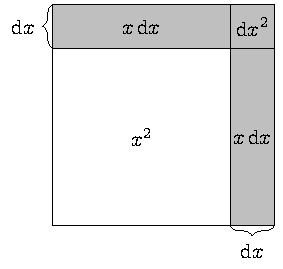
\includegraphics{basicderivativesandintegrals/xsquaredpowerrule}
	\caption{Interpretation of $\odv{x^2}{x}$ ($\odif{x}$ exaggerated)}
    \label{fig:xsquaredpowerrule}
\end{figure}
Illustrated in \cref{fig:xsquaredpowerrule},
\begin{equation}
    \odv*{(x^2)}{x} = \lim_{\odif{x} \appr 0} \frac{x\odif{x} + x\odif{x} + \odif{x}^2}{\odif{x}}. \label{eq:xsquaredpowerrule}
\end{equation}
When $\odif{x} \appr 0$, the $\odif{x^2}$ square would just become a single point. Compared to the big $x\odif{x}$ on the side, it's negligible; therefore, we can safely ignore it. The equation then becomes
\begin{align*}
    \odv*{(x^2)}{x} = \lim_{\odif{x} \appr 0}\frac{2x\odif{x}}{\odif{x}} = 2x,
\end{align*}
which is equivalent to the result from the power rule.

Deriving $\odv*{(x^3)}{x}$ geometrically shouldn't be too hard either. Take a cube sidelength $x$; increase its side length by $\odif{x}$, and compute the ratio between the change in volume and $\odif{x}$. The final answer should be $3x^2$. You could try with more higher order of $n$, but it'd be very hard to visualize.

Here I leave some exercises which shouldn't be too hard to do
\begin{enumerate}
    \item $\odv*{(x^2 - 2x + 16)}{x}$ \hfill $2x - 2$
    \item $\odv*{(x^3 + x^2 + x + 1)}{x}$ \hfill $3x^2 + 2x + 1$
    \item $\odv*{(3x^4 + 24x^3 - 2x^2 - 32x + 88)}{x}$ \hfill $12x^3 + 72x^2 - 4x - 32$
\end{enumerate}

\subsection{Antiderivatives of polynomials: the reversed power rule}

For the antiderivative of $x^n$, we use the fundamental theorem of calculus (\cref{theorem:fundamentalthmofcalc1}) on the power rule (\cref{eq:power_rule}),
\begin{equation*}
    x^n = \int nx^{n - 1} \odif{x}.
\end{equation*}
Substitute $n$ with $n + 1$
\begin{equation*}
    \int (n + 1)x^{n}\odif{x} = x^{n + 1} + C,
\end{equation*}
and by the linearity of integrations (\cref{eq:integralsconstantmultiple}), we get the \index{integrals!reversed power rule}\textbf{reversed power rule}:
\begin{equation}
	\int x^{n}\odif{x} = \frac{x^{n + 1}}{n + 1} + C. \label{eq:reversed-power-rule}
\end{equation}

Notice, this rule does not work for $n = 1$ because we can't divide by zero\dots \emph{or can we???} (Discussed further in \cref{sec:integralofthereciprocal})

\subsection{Extending the equations of linear motion}

Let's use the power rule to extend the equation of linear motions in \cref{sec:fiveequationsoflinearmotion} to include a constant jerk $j$, i.e.,
\begin{equation}
    \odv{a}{t} = j
\end{equation}
Then, we can move the $\odif{t}$ around and integrate both sides by using the reversed power rule.
\begin{align*}
    \int j\odif{t} &= \int\odif{a} \\
    j\int \odif{t} &= \int\odif{a} \alc[0.3]{Linearity of integrals} \\
    jt + a_0 &= a \alc[0.3]{Integral constant $a_0$}
\end{align*}
Because $a$ is the derivative of $v$, 
\begin{align*}
    \odv{v}{t} &= jt + a_0 \\
    \int \odif{v} &= \int jt + a_0 \odif{t} \\
    v &= j\int t\odif{t} + \int a_0\odif{t} \alc{Linearity of integrals} \\
    v &= \frac{1}{2}jt^2 + a_0t + v_0. \alc{Reversed power rule}
\end{align*}
We add $v_0$ as an integral constant in a similar manner. Since $v$ is the derivative of $r$,
\begin{align*}
    \odv{r}{t} &= \frac{1}{2}jt^2 + a_0t + v_0 \\
    \int \odif{r} &= \int\frac{1}{2}jt^2 + a_0t + v_0 \odif{t} \\
    r &= \frac{1}{2}j\int t^2\odif{t} + a_0\int t\odif{t} + v_0\int\odif{t} \\
    r &= \frac{1}{6}jt^3 + \frac{1}{2}a_0t^2 + v_0t + r_0.
\end{align*}
And there you have it! Further extensions can be made from here: the jerk could be time-dependent. But that's probably enough to illustrate my point. If you'd like to try, extend the equation of motion to have a constant snap: $\odv{j}{t} = s$. You should get
\begin{equation*}
    r = \frac{1}{24}st^4 + \frac{1}{6}jt^3 + \frac{1}{2}a_0t^2 + v_0t + r_0.
\end{equation*}

\section{Exponentials and growth}

\begin{wraptable}[15]{l}{0.445\textwidth}
    \centering
    \begin{tabular}{C | C | C}
        t & V(t) & V(t) - V(t - 1) \\
        \hline
        0 & 1 & \\
        1 & 2 & 2 - 1 = 1 \\
        2 & 4 & 4 - 2 = 2 \\
        3 & 8 & 8 - 4 = 4 \\
        4 & 16 & 16 - 8 = 8 \\
        5 & 32 & 32 - 16 = 16 \\
        6 & 64 & 64 - 32 = 32 \\
        7 & 128 & 128 - 64 = 64 \\
        8 & 256 & 256 - 128 = 128 \\
        9 & 512 & 512 - 256 = 256 \\
        10 & 1024 & 1024 - 512 = 12
    \end{tabular}
    \caption{Tables of $2^x$ plotted at interval $1$ from $0$ to $10$}
    \label{tab:exponentialbase2}
\end{wraptable}
The next function that we're going to discuss is exponentials: the mathematical representation of growth and decay. As an example, let's say there's a magical drop of water that doubles its volume $V$ every hour. I.e., for any time $t$,
\begin{equation}
    V(t + 1) = 2V(t). \label{eq:exponentialsrecurrencerelations}
\end{equation}
If the drop starts at one unit of volume, $V(0) = 1$; thus,
\begin{align*}
    V(1) &= 2V(0) = 2, \\
    V(2) &= 2V(1) = 2(2) = 2^2, \\
    V(3) &= 2V(2) = 2(2^2) = 2^3, \\
    V(4) &= 2V(3) = 2(2^3) = 2^4, \\
    &\vdots
\end{align*}
It's clear that the pattern is $V(t) = 2^t$: an exponential function. A natural question to ask is ``\emph{what is its rate of change?}''. Let's start by plotting the function over time (\cref{fig:exponentialgraph}). But, exponentials grow too quick to plot! By $V(7)$, we're already in the hundreds. So It'd probably be better to list the values of each point on a table.
\begin{figure}[t]
    \centering
    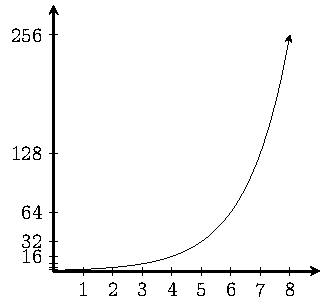
\includegraphics{basicderivativesandintegrals/exponentials}
    \caption{Exponential function $2^x$ plotted from $0$ to $8$}
    \label{fig:exponentialgraph}
\end{figure}
Notice that on the right most column of \cref{tab:exponentialbase2}, the difference between $V(t)$ and $V(t - 1)$ is exactly $V(t - 1)$: the function changes as much as its past-self. So does that mean that $\odv*{(2^x)}{x} = 2^x$?

Well sadly not, but close. See, \cref{tab:exponentialbase2} only shows a \emph{discrete} step. You can write it out as
\begin{equation}
    \frac{2^{x + 1} - 2^x}{1} = 2^x\left(\frac{2 - 1}{1}\right) = 2^x,
\end{equation}
that is why $V(t) - V(t - 1) = V(t - 1)$. But we still need the method of increments to calculate the derivative of $2^x$:
\begin{align*}
    \odv*{(2^x)}{x} &= \lim_{h \appr 0}\frac{2^{x + h} - 2^x}{\odif{x}} \\
    &= 2^x\lim_{h \appr 0}\left(\frac{2^h - 1}{h}\right).
\end{align*}
Now you could try plugging in a really small value of $h$, say $0.000001$. The term $\frac{2^h - 1}{h}$ will approach $0.69314\dots$. If you try other bases of exponents, say $3$, you might see a pattern emerging.
\begin{equation}
    \odv*{(3^x)}{x} = 3^x\lim_{h \appr 0}\frac{3^h - 1}{h}.
\end{equation}
\emph{The rate of change of an exponential function is always itself times a proportionality constant}. For $3^x$, it's about $1.09851\dots$. If we could find a number $n$ where $\frac{n^h - 1}{h} = 0$, we'd have a very pretty function which it is its own derivative. So let's find that!
 
\subsection{A function that is its own derivative}
\label{sec:function_equals_own_derivative}

Let's set a goal: find the function that is its own derivative. I shall introduce a substantial concept in calculus: the expansion of functions. Every function has a polynomial expansion\footnote{Although the convergence of the series derived is quite questionable; thankfully, the power series of $n^x$ converges everywhere.} called the \index{power series!introduction}\textbf{power series}. For every $f(x)$,
\begin{equation}
    f(x) = a_0 + a_1x^1 + a_2x^2 + a_3x^3 +\dots. \label{eq:naivetaylorseries}
\end{equation}
E.g., $\sin(x)$ can be written as
\begin{equation}
    \sin(x) = x - \frac{1}{3!}x^3 + \frac{1}{5!}x^5 - \frac{1}{7!}x^7 + \dots. \label{eq:taylorseriessine}
\end{equation}
we will derive this expression later in \cref{sec:sine_cosine_power_series}. For now, we can just use \cref{eq:naivetaylorseries} to find the expression for the function that is its own derivative.

We've seen that the exponential is a possible candidate for a function that is its own derivative. Now, assume that for some real number $n$,
\begin{equation}
    \odv*{(n^x)}{x} = n^x.
\end{equation}
Then, we use the polynomial expansion and the power rule,
\begin{align*}
    \odv*{(a_0 + a_1x^1 + a_2x^2 + a_3x^3 + \dots)}{x} &= a_1 + 2a_2x^1 + 3a_3x^2 + 4a_4x^3 + \dots \\
    &= n^x
\end{align*}
If the function is its own derivative, the polynomial expansion of the function and its derivative must be the same.
\begin{gather}
    n^x = a_0 + a_1x^1 + a_2x^2 + a_3x^3 + \dots, \label{eq:naivetaylorseries1}\\
    n^x = a_1 + 2a_2x^1 + 3a_3x^2 + 4a_4x^3 + \dots. \label{eq:naivetaylorseries2}
\end{gather}
Since both are polynomials, we can match the coefficient here:
\begin{equation}
    \begin{array}{c}
    a_0 = a_1 \\ a_1 = 2a_2 \\ a_2 = 3a_3 \\ a_3 = 4a_4 \\ \vdots
    \end{array}\label{eq:naivetaylorserieserelations}
\end{equation}
$a_0$ and $a_1$ is relatively easy to find. As we've seen, $n$ must be between $2$ and $3$. By the properties of exponentials, $x = 0 \implies n^x = 1$. We can then plug $x = 0$ and set $n^x = 1$ into \cref{eq:naivetaylorseries2}:
\begin{align*}
    1 &= a_0 + a_1(0)^1 + a_2(0)^2 + a_3(0)^3 + \dots \\
    a_0 &= 1.
\end{align*}
Since $a_0 = a_1$, $a_1$ must also be $1$. We can then go back to \cref{eq:naivetaylorserieserelations} and get
\begin{equation*}
    n^x = 1 + 1 + \frac{1}{2!}x + \frac{1}{3!}x^3 + \frac{1}{4!}x^4 + \dots
\end{equation*}
The pattern here is clearly $a_n = n!$. If we want to find $n$, we just let $x = 1$.
\begin{equation*}
    n = 1 + 1 + \frac{1}{2!} + \frac{1}{3!} + \frac{1}{4!} + \dots,
\end{equation*}
and there we have an expression for $n$ which is an irrational number. If you work this out, it's around $2.71828\dots$. Because $(2.71828\dots)^x$ is its own derivative, it's very useful in mathematics and appears everywhere, even at the seams of mathematics that doesn't even seems related to growths: the patterns of prime number, this constant $2.71828\dotso$ has a name and symbol: the Euler's number\footnote{Not to be confused with the ``Euler's constant'' which is another constant written $\gamma$, and is around $0.57721\dots$}, written as $\e$ where
\begin{equation}
    \e = \sum_{i = 0}^{\infty}\frac{1}{i!}
\end{equation}

\subsection{\protect Another interpretation of $\e$: infinite bank interests}

There are two types of bank interests: simple and compound. Simple interests is the thing that you don't really want: the interest is always the same and doesn't grow with your account. You can calculate it by using
\begin{equation}
    n(t) = n_0 + tr
\end{equation}
where $n(t)$ is the total money at time $t$, $n_0$ the initial money in your bank account, and $r$, the interest rate.

Compound interest in the other hand calculates your interest based on how much money you have at that moment:
\begin{equation}
    n(t + 1) = n(t)r + n(t).
\end{equation}
We can find the expression for $n(t)$ in a similar fashion to what we've done in \cref{eq:exponentialsrecurrencerelations}. You'll get
\begin{equation}
    n(t) = (1 + r)^tn_0 \label{eq:compoundinterestformula}
\end{equation}
which is an exponential function.

Let's say you deposit $100\$$ into a bank and the bank is offering you two options on \index{compound interest}\textbf{compound interests} rate. \begin{enumerate*}[label = \arabic*)]\item Take $100\%$ interest in $1$ year, \item Take $\flatfrac{100}{2}\%$ twice a year, or \item Take $\flatfrac{100}{356}\%$ daily.\end{enumerate*} If you take option one, you'd end up with $200\$$. Option two takes you to $225\$$, and option three takes you to around $271.447\dots\$$. You might see a theme here. If you get $\flatfrac{100}{n}\%$ interest, $n$ times a year, the result keeps getting higher. Is there an upper limit to this?

If we write it in terms of limits as $n \appr \infty$ and use \cref{eq:compoundinterestformula}, the compound interests formula,
\begin{equation*}
    x = \lim_{n \appr \infty}\left(1 + \frac{1}{n}\right)^nn_0.
\end{equation*}
Where $x$ is the total money after a year. We're interested in the upper limit, so we'll just let $n_0$ for now. The expression will become
\begin{equation}
    x = \lim_{n \appr \infty}\left(1 + \frac{1}{n}\right)^n \label{eq:infinitecompoundinterest}
\end{equation}
Technically, we could go in and substitute a very high $n$, such as $1000000$. But I believe you could already see that it would be a nightmare to calculate: exponentiation is not at all an easy task. However, notice that from option three earlier, the total money is $271.447\dots\$$ which is suspiciously similar to $\e$ at $2.71828\dots$. If \cref{eq:infinitecompoundinterest} equals \cref{eq:naivetaylorserieserelations}, we'd find the upper limit for this problem and solve the mystery.

We can use the binomial theorem on \cref{eq:infinitecompoundinterest} and get
\begin{align*}
    &\lim_{n \appr \infty}\sum_{k = 0}^{n}{n \choose k}1^{n - k}\frac{1}{n^k} \\
    &= \lim_{n \appr \infty}{n \choose 0}\frac{1}{n^0} + {n \choose 1}\frac{1}{n^1} + {n \choose 2}\frac{1}{n^2} + {n \choose 3}\frac{1}{n^3} + \dots.
\end{align*}
Then, we use the definition of $n$ choose $k$,
\begin{align*}
    &= 1 + \lim_{n \appr \infty}\frac{n!}{1!(n - 1)!}\frac{1}{n^1} + \frac{n!}{2!(n - 2)!}\frac{1}{n^2} + \frac{n!}{3!(n - 3)!}\frac{1}{n^3} + \dots.
\end{align*}
Now, we can cancel the $n!$ on the numerator to the denominator and isolate the factorials.
\begin{align*}
    &= 1 + \lim_{n \appr \infty}\frac{n(n - 1)!}{(n - 1)!}\frac{1}{1!n^1} + \frac{n(n - 1)(n - 2)!}{(n - 2)!}\frac{1}{2!n^2} + \dots \\
    &= 1 + \frac{1}{1!} + \lim_{n \appr \infty} \frac{n(n - 1)}{2!n^2} + \frac{n(n - 1)(n - 2)}{3!n^3} + \frac{n(n - 1)(n - 2)(n - 3)}{4!n^4} + \dots
\end{align*}
Notice, as $n \appr \infty$, the ratio between $n + R$ and $n$ where $R$ is any real numbers would be literally negligible. For every terms in our series, both the numerator and the denominator has the same polynomic degrees. Therefore, all the $n$'s in the series cancel out and we get
\begin{equation}
    x = 1 + \frac{1}{1!} + \frac{1}{2!} + \frac{1}{3!} + \dots
\end{equation}
which is literally \cref{eq:naivetaylorserieserelations}; thus,
\begin{equation}
	\e = \lim_{n \appr \infty}\ab(1 + \frac{1}{n})^n. \label{eq:e-def-infinite-interests}
\end{equation}

In conclusion, the upper limit that the bank can give you is $\e$, which should make sense geometrically. Because we're gradually turning a discrete interest into a continuous one, $\e$ should appear in the limit of the continuous bank interests.

The limit definition of $\e$ allows us to express $\e^x$ in terms of limits.
\begin{align}
	\e^x &= \ab(\lim_{n \appr \infty}\ab(1 + \frac{1}{n})^n) \\
		 &= \lim_{n \appr \infty}\ab(1 + \frac{1}{n})^{nx}
\end{align}
If $n = \flatfrac{u}{x}$, then
\begin{align}
	\e^x &= \lim_{\frac{u}{x} \appr \infty}\ab(1 + \frac{u}{h})^{h}
\end{align}
For $\frac{u}{x} \appr \infty$ to be true for all finite $x$, $u$ must approach $\infty$; therefore,
\begin{align}
	\e^x &= \lim_{u \appr \infty}\ab(1 + \frac{u}{h})^h
\end{align}

\subsection{The antiderivative of exponential functions}

It should be trivial that if $\e^x$ is the derivative of itself, so is its antiderivative
\begin{equation}
    \int \e^x \odif{x} = \e^x + C.
\end{equation}
For other bases, we could use the fundamental theorem of calculus (\cref{theorem:fundamentalthmofcalc1}) to find its antiderivative. I.e., if
\begin{equation*}
    \odv{(n^x)}{x} = n^x\lim_{h \appr 0}\frac{n^h - 1}{h},
\end{equation*}
then
\begin{align*}
    \odv*{(n^x)}{x} &= n^x\lim_{h \appr 0}\frac{n^h - 1}{h} \\
    n^x &= \lim_{h \appr 0}\frac{n^h - 1}{h}\int n^x\odif{x} \\
    \int n^x\odif{x} &= n^x\lim_{h \appr 0}\left(\frac{n^h - 1}{h}\right)^{-1} + C.
\end{align*}
The term in the limit sign still appears here. If we want to uncover the origin of this term, we must discuss the logarithms.

\section{Logarithms}

Logarithms are inverses of exponential, like how roots are inverses of monomials. To illustrate what I mean,
\begin{equation*}
	\textrm{For monomials, } \sqrt[a]{x^a} = x, \textrm{ but with logarithms, } \log_{a}(a^x) = x.
\end{equation*}
They have the following properties:
\begin{gather}
    \log_a(x) + \log_a(y) = \log_a(xy), \\
    \log_a(x) - \log_a(y) = \log_a\left(\frac{x}{y}\right), \\
    \log_a(x) = \frac{\log_b(x)}{\log_b(a)}.
\end{gather}
Since $\e^x$ is shown to be a very important function in modelling continuous growth, and is its own derivative, we give its inverse function its own name: the \index{logarithms!natural logarithms}\textbf{natural logarithm}, written as $\ln(x)$.

What's the derivative of $\ln(x)$? By the method of increments,
\begin{align}
	\odv*{\ln(x)}{x} &= \lim_{h \appr 0}\frac{\ln(x + h) - \ln(x)}{h} \\
					&= \lim_{h \appr 0}\frac{\ln(\frac{x + h}{x})}{h} \\
					&= \lim_{h \appr 0}\frac{\ln(1 + \frac{h}{x})}{h} \\
					&= \lim_{h \appr 0}\ln\ab(\ab(1 + \frac{h}{x})^{\frac{1}{h}}).
\end{align}
This form is very similar to the limit definition of the exponential function $\e^x$, but with some terms swapped around. So let's try to fit this limit to the form of $\e^x$. I shall let $h = \frac{1}{n}$. If $h \appr 0$, then $n \appr \infty$. Therefore,
\begin{align}
	\odv*{\ln(x)}{x} &= \lim_{n \appr \infty}\ln\ab(\ab(1 + \frac{1}{nx})^{n}) \\
					 &= \lim_{n \appr \infty}\ln\ab(\ab(1 + \frac{\flatfrac{1}{x}}{n})^n). \label{eq:ln-diff-derivation}
\end{align}
Recall that
\begin{equation}
	\e^x = \lim_{n \appr \infty}\ab(1 + \frac{x}{n})^n.
\end{equation}
Thus,
\begin{equation}
	\lim_{n \appr \infty}\ab(1 + \frac{\flatfrac{1}{x}}{n})^n = \e^{\frac{1}{x}}.
\end{equation}
which fits the form of \cref{eq:ln-diff-derivation}. Therefore,
\begin{align}
	\odv*{\ln(x)}{x} &= \lim_{n \appr \infty}\ln(\e^{\frac{1}{x}}) \\
					 &= \lim_{n \appr \infty}\frac{1}{x} = \frac{1}{x}:
\end{align}
the derivative of the natural logarithm of $x$ is the reciprocal of $x$.

This result can also be interpretted geometrically. If the exponential grows very quickly when $x$ increases, its inverse must grow slow. The slow growing rate is directly captured by the function $\frac{1}{x}$.

Here is the perfect time that I'll give you a glimpse into calculus with many variables: multivariable calculus. I shall present another way to derive the derivative of $\ln(x)$: \textbf{implicit differentiation}.\index{implicit differentiation}

Functions in the form $f(x) = y$ are called \textbf{explicit functions}: the relations between the two variables are written explicitly. Functions that can't be written as $f(x) = y$ are called \textbf{implicit functions}, e.g., $x^2 + y^2 = r^2$. \textbf{Implicit differentiation} concerns the differentiation of implicit functions. In this case, it actually makes our life easier if we turn $\ln(x)$ into an implicit function.

If I let $\ln(x) = y$, I can raise both sides to the power of $\e$ and get
\begin{equation}
    \e^{\ln(x)} = \e^y.
\end{equation}
Because logarithms are inverses of exponential,
\begin{equation}
    x = \e^y.
\end{equation}
By the rule of equality, (\cref{sec:trivial_rules}), we can take the derivative of both sides w.r.t. $y$ instead of $x$:
\begin{align*}
    \odv{x}{y} &= \odv{\e^y}{y} \\
    \odv{x}{y} &= \e^y.
\end{align*}
But we're looking for the derivative of $y$ (which is just $\ln(x)$) w.r.t. $x$, not the derivative of $x$ w.r.t. $y$. Here's where Leibniz's notation comes into clutch: we can swap the numerator with the denominator for both sides then, substitute back $y = \ln(x)$:
\begin{align*}
    \odv{\ln(x)}{x} &= \frac{1}{\e^{\ln(x)}} \\
    \therefore~\odv{\ln(x)}{x} &= \frac{1}{x},
\end{align*}
and there: the derivative of the natural logarithm is the reciprocal.

With the power of natural logarithms, we can actually go back at the derivative of $n^x$ and finally uncover the mystery behind the proportionality term that's lingering around. Start with the manipulation of $n^x$.
\begin{equation}
    n^x = \left(\e^{\ln(n)}\right)^x = \e^{x\ln(x)}.
\end{equation}
With the chain rule (\cref{sec:trivial_rules}), let $u = x\ln(n)$:
\begin{align*}
    \odv*{(n^x)}{x} &= \odv{\e^{x\ln(n)}}{x} \\
    &= \odv{\e^u}{x} \times \odv{u}{u} \\
    &= \odv{\e^u}{u} \times \odv{u}{x} \\
    &= \e^{x\ln(n)} \times \odv{x\ln(n)}{x} \\
    &= n^x\ln(n).
\end{align*}
And here it is: the mystery proportionality constant. It's just a consequence of the natural logarithm. Thus, one way to define the natural log would be
\begin{equation}
    \ln(n) = \lim_{h \appr 0}\frac{n^h - 1}{h}.
\end{equation}
The antiderivative of other bases exponents are then given by
\begin{equation}
    \int n^x = \frac{1}{\ln(n)}n^x + C.
\end{equation}

\subsection{The product rule and the quotient rule}
\index{derivatives!product rule}

Sometimes, we have to multiply the two functions together before taking the derivatives. There are two ways to do this. To keep the spirit of visualization, I shall first introduce the geometrical way, then the analytical way.

\begin{figure}[h]
    \centering
    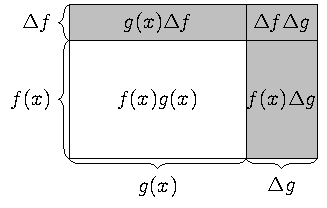
\includegraphics{basicderivativesandintegrals/derivativesproductrule}
    \caption{The geometrical interpretation of the product rule.}
    \label{fig:derivativesproductrule}
\end{figure}
The derivative of $f(x)g(x)$ w.r.t. $x$ can be thought of a rectangle with side length that's governed by $f(x)$ and $g(x)$. As shown in \cref{fig:derivativesproductrule}, the area increase on side $f(x)$ is $g(x)\Dd{f}$ and on $g(x)$, $f(x)\Dd{g}$. The $\Dd{f}\Dd{g}$ part is basically negligible. Therefore,
\begin{align*}
    \odv*{\ab(f(x)g(x))}{x} &= \lim_{h \appr 0}\frac{g(x)\Dd{f} + f(x)\Dd{g}}{h} \\
    &= \lim_{h \appr 0}\frac{f(x)(g(x + h) - g(x)) + g(x)(f(x + h) - f(x))}{h} \\
    &= f(x)\lim_{h \appr 0}\frac{g(x + h) - g(x)}{h} + g(x)\lim_{h \appr 0}\frac{f(x + h) - f(x)}{h} \\
    &= f(x)\odv{g(x)}{x} + g(x)\odv{f(x)}{x}.
\end{align*}
Which is what we call the product rule. Notice the alternation between $f$ and $g$ in the two terms. The derivative of $f(x)$ is multiplied by $g(x)$, and the derivative of $g(x)$ is multiplied by $f(x)$. This is a direct consequence of the diagram: the change in $f(x)$ is multiplied by $g(x)$ to give the area and also the other way around. You could check this with the method of increments, and it would still be true. I encourage you to do it.

\index{derivatives!quotient rule}To take derivatives of quotients of functions, just plug in $\flatfrac{1}{g(x)}$ instead of $g(x)$. The final form should be
\begin{equation}
    \odv*{\ab(\frac{f(x)}{g(x)})}{x} = \frac{\displaystyle f(x)\odv{g(x)}{x} - g(x)\odv{f(x)}{x}}{f(x)^2}.
\end{equation}
But how's about the product of multiple functions? We can't really geometrically interpret those anymore. So we have to turn ourselves to the analytical method.

Let's think of this through. We don't know the derivative of products, but we know the derivative of \emph{sums}: the linearity property. So if we can turn products into sum, this problem would be so easy! Gladly, the logarithms can do exactly that. To make our life easier, we shall use the natural logarithm. Because I want to save space, let's write $a(x)b(x)c(x)$ as just $abc$. Do know that these functions are all dependent on $x$. Start off with a manipulation of products.
\begin{align*}
    \odv{(abc\dots)}{x} &= \odv*{(\e^{\ln(abc\dots)})}{x} \\
    &= \odv*{(\e^{\ln(a) + \ln(b) + \ln(c) + \dots})}{x}.
\end{align*}
Now, let $\ln(a) + \ln(b) + \ln(c) + \dots = u$ and use the chain rule,
\begin{align*}
    &= \odv*{(\e^u)}{x} \cdot \odv{u}{u} \\
    &= \odv*{(\e^u)}{x} \cdot \odv*{\ab(\ln(a) + \ln(b) + \ln(c) + \dots)}{x} \\
    &= \e^u \left(\odv{\ln(a)}{x} + \odv{\ln(b)}{x} + \odv{\ln(c)}{x} + \dots\right).
\end{align*}
Then use the chain rule again on the terms in the parenthesis
\begin{align*}
    &= \e^u \left(\odv{\ln(a)}{x}\odv{a}{a} + \odv{\ln(b)}{x}\odv{b}{b} + \odv{\ln(c)}{x}\odv{c}{c} + \dots\right) \\
    &= (abc\dots)\left(\odv{\ln(a)}{a}\odv{a}{x} + \odv{\ln(b)}{b}\odv{b}{x} + \odv{\ln(c)}{c}\odv{c}{x} + \dots\right) \\
    &= (abc\dots)\left(\frac{1}{a}\odv{a}{x} + \frac{1}{b}\odv{b}{x} + \frac{1}{c}\odv{c}{x} + \dots\right).
\end{align*}
And there we have it: the generalized product rule.

\subsection{Alternative derivations for the power rule}

The power rule can also be derived using the same technique we just used. However, we use a different property of logarithm: $\ln(x^n) = n\ln(x)$.
\begin{equation*}
    \odv*{x^n}{x} = \odv*{\e^{n\ln(x)}}{x}.
\end{equation*}
Let $u = n\ln(x)$ then use the chain rule
\begin{align*}
    &= \odv{\e^u}{x} \cdot \odv{u}{u} \\
    &= \odv{\e^u}{u} \cdot \odv{u}{x} \\
    &= \e^u \cdot \odv*{\ab(n\ln(x))}{x} \\
    &= x^n \cdot n\frac{1}{x} = nx^{n - 1}.
\end{align*}

\section{Implicit differentiation}

Implicit differentiation also shows up in problems where two rate of changes are related to each other: the \textbf{related rates} problem. Consider a sliding ladder that's $5\unit{\meter}$ long (\cref{fig:slidingladder}). At a certain time $t$, what's the sliding rate along the $x$-axis w.r.t. the $y$-axis?\index{related rates}

\begin{figure}
    \centering
    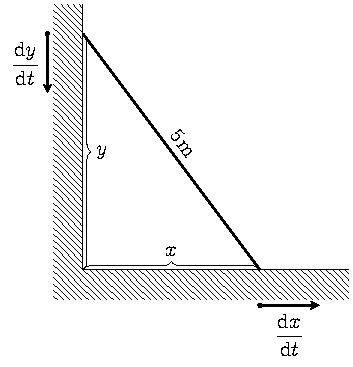
\includegraphics{basicderivativesandintegrals/slidingladder}
    \caption{A ladder length $5\unit{\meter}$ sliding down a corner.}
    \label{fig:slidingladder}
\end{figure}

The problem is asking for $\odv{x}{y}$. Here, the rate of sliding along the $y$-axis $\odv{y}{t}$ and along the $x$-axis $\odv{x}{t}$ is related because the ladder length is fixed. If $y$ decreases, $x$ must increase. The Pythagorean theorem says
\begin{equation}
    x^2 + y^2 = 5^2.
\end{equation}
We can take the derivative w.r.t. $t$ on both side then use the chain rule
\begin{align*}
    \odv{x^2}{t} + \odv{y^2}{t} &= \odv{(5^2)}{t} \\
    \odv{x^2}{x}\odv{x}{t} + \odv{y^2}{y}\odv{y}{t} &= 0 \\
    2x\odv{x}{t} + 2y\odv{y}{t} &= 0.
\end{align*}
We can take advantage of the Leibniz's notation and multiply by $\odif{t}$ on both sides giving
\begin{equation*}
    2x\odif{x} + 2y\odif{y} = 0.
\end{equation*}
To find $\odv{x}{y}$, we just have to isolate the variables,
\begin{align*}
    \odv{x}{y} = -\frac{y}{x}.
\end{align*}
And this should actually make sense. Because if $y$ is increasing by a bit, $x$ must decrease by some amount, and that amount is $-\flatfrac{y}{x}$: the higher the $y$, the larger the rates of sliding.

\section{Technique of integraton: substitution}

Before we finish this chapter off, I'd want to take a look at a very useful technique for dealing with complicated integrals: substitution.

Substitution is a technique to simplify algebraic expressions. I believe you've already seen a multitude of them. Basically, we substitute some expression of $x$ with $u$, then use everything in our power to change every $x$ to $u$, including the differential element: from $\odif{x}$ to $\odif{u}$.

$u$-substitution works when the integrals are of the form
\begin{equation}
	\int f\ab(g(x))\odv{g(x)}{x}\odif{x}.
\end{equation}
In this notation, it's easy to see that the $\odif{x}$ will cancel, leaving us with
\begin{equation}
	\int f\ab(g(x))\odif{g(x)}.
\end{equation}
If $g(x) = u$, then our integral simplifies to
\begin{equation}
	\int f(u)\odif{u}.
\end{equation}

Let's apply this knowledge to solve some integrals. Starting with the simplest: polynomic integrands.
\begin{exmp}{$\int x(x^2 + 1)^{10}\odif{x}$}{u-substitution-1}
	If $f(x) = x^{10}$, and $u = x^2 + 1$, then
	\begin{equation}
		\int x(x^2 + 1)^{10}\odif{x} = \int u^{10}x\odif{x}.
	\end{equation}
	Because $x = \frac{1}{2}\odv{(x^2 + 1)}{x}$,
	\begin{equation}
		\int u^{10}x\odif{x} = \int u^{10}\frac{1}{2}\odv{(x^2 + 1)}{x}\odif{x} = \frac{1}{2}\int u^{10}\odif{(x^2 + 1)}
	\end{equation}
	Since $u = x^2 + 1$, our integral simplifies to
	\begin{equation}
		\frac{1}{2}\int u^{10}\odif{u}.
	\end{equation}
	Using the reversed power rule (\cref{eq:power_rule}), we get
	\begin{equation}
		\frac{1}{2}\frac{u^{11}}{11} = \frac{u^{11}}{22} = \frac{(x^2 + 1)^{11}}{22} + C.
	\end{equation}
\end{exmp}

\begin{exmp}{$\int x^2\e^{4x^3 + 4}\odif{x}$}{u-substitution-3}
	The integrand is a composite function: $f(u) = \e^u$ and $u = 4x^3 + 4$. In which, $\odv{u}{x} = 12x^2$; therefore,
	\begin{align}
		\int x^2\e^{4x^3 + 4}\odif{x} &= \frac{1}{12}\int\e^u 12x^2 \odif{x} \\
										&= \frac{1}{8}\int\e^u\odv{u}{x}\odif{x} \\
										&= \frac{1}{8}\int\e^u\odif{u} = \frac{1}{8}\e^u \\
										&= \frac{1}{12}\e^{4x^3 + 4} + C.
	\end{align}
\end{exmp}

Notice any patterns? If the integral has a polynomial $u$ with degree $n$ nested inside another function, there must be a term outside with the degree $n - 1$ to substitute with. In \cref{exmp:u-substitution-1}, $u = x^2 + 1$ and there's an $x$ multiplied outside waiting to be substituted. In \cref{exmp:u-substitution-3}, $u = 4x^3 + 4$, and there's an $x^2$ outside. This pattern is a consequence of the power rule, and is pretty common. So, here are some practice problems with answers and hints on the right.\footnote{Practice problems taken from \cite{foster-no-date}.} Try not to look at it much.

\begin{enumerate}
	\item $\int 3x^2\sqrt{x^3 + 5}\odif{x}$ \hfill $\frac{2}{3}(x^3 + 5)^{\frac{3}{2}} + C$, $u = x^3 + 5$
	\item $\int \sqrt{4 + 3x}\odif{x}$ \hfill $\frac{2}{9}(3x + 4)^{\frac{3}{2}} + C$, $u = 4 + 3x$
	\item $\int \frac{24x}{(4x^2 + 4)^2}\odif{x}$ \hfill $\frac{3}{4x^2 + 4} + C$, $u = 4x^2 + 4$
\end{enumerate}

Now let's move on from polynomials to other functions that are nested inside another function. For the substitution to work, there must be the function's derivative multiplied, waiting to be substituted. A classic example is:
\begin{exmp}{$\int \frac{\ln(x)}{x}\odif{x}$}{u-substitution-3}
	This integral is not quite a composite function, but rather just a product between a function and its derivative. If $u = \ln(x)$, then $\odv{u}{x} = \frac{1}{x}$; therefore,
	\begin{align}
		\int \frac{\ln(x)}{x}\odif{x} &= \int u\odv{u}{x}\odif{x} \\
									  &= \int u\odif{u} \\
									  &= \frac{u^2}{2} = \frac{\ln(x)^2}{2} + C.
	\end{align}
\end{exmp}

\begin{exmp}{$\int x\e^{x^2}(\e^{x^2} + 3)\odif{x}$}{u-substitution-4}
	Let $\e^{x^2} + 3 = u$, then
	\begin{align}
		\odv{u}{x} &= \odv{\e^{x^2} + 3}{x} \\
				   &= \odv{\e^{x^2}}{x} \\
				   \intertext{Let $x^2 = v$, then by the chain rule,}
				   &= \odv{\e^v}{x} \cdot \odv{v}{v} \\
				   &= \odv{\e^v}{v} \cdot \odv{x^2}{x} \\
				   &= 2x\e^v = 2x\e^{x^2}.
	\end{align}
	Thus,
	\begin{align}
		\int x\e^{x^2}(\e^{x^2} + 3)\odif{x} &= \frac{1}{2}\int u\ab(2x\e^{x^2})\odif{x} \\
											 &= \frac{1}{2}\int u\odv{u}{x}\odif{x} = \frac{1}{2}\int u\odif{u} \\
											 &= \frac{1}{2}\frac{u^2}{2} = \frac{(\e^{x^2} + 3)^2}{4} + C.
	\end{align}
\end{exmp}

Sometimes, they need some \emph{creative} algebraic manipulations, and sometimes even multiple substitution. E.g.,\footnote{Taken from MIT Integration Bee 2019, $I_9$ \cite{alkousa-2023}}
\begin{exmp}{$\frac{1}{x(x^5 + 1)}\odif{x}$}{u-substitution-5}
	If we want to use power rule substitution, there's only $x^5$ but no $x^4$ to substitute with. So, we need to get a bit creative.

	First, factor the $x^5$ out of the inner parenthesis and get
	\begin{equation}
		\int\frac{1}{x^6\ab(1 + \frac{1}{x^5})}\odif{x}.
	\end{equation}
	Now, we can let $u = 1 + \frac{1}{x^5}$. By the power rule, $\odv{u}{x} = -\frac{5}{x^6}$. Our integral then becomes
	\begin{align}
		-5\int\frac{1}{u}\ab(-\frac{5}{x^6})\odif{x} &= -\frac{1}{5}\int\frac{1}{u}\odv{u}{x}\odif{x} \\
													 &= -\frac{1}{5}\int\frac{1}{u}\odif{u} = -5\ln(x) \\
													 &= -\frac{1}{5}\ln\ab(1 + \frac{1}{x^5}) + C
	\end{align}
\end{exmp}

In certain problems, there aren't any outside terms to substitute with, so you have to create them. E.g.,
\begin{exmp}{$\int\ab(1 + \sqrt{x})^4\odif{x}$}{}
	We want to get rid of the term inside the parenthesis. So, let $u = 1 + \sqrt{x}$, and by the power rule, $\odv{u}{x} = \frac{1}{2\sqrt{x}}$. However, there is no $\frac{1}{\sqrt{x}}$ outside to substitute with. Let's be adventurous and substitute $u$ in anyways and see what happens.
	\begin{align}
		\int(1 + \sqrt{x})^4\odif{x} &= \int u^4\odif{x}
		\intertext{If $\odv{u}{x} = \frac{1}{2\sqrt{x}}$, then $\odif{x} = 2\sqrt{x}\odif{u}$,}
									 &= \int u^4\ab(2\sqrt{x})\odif{u}.
	\end{align}
	We're almost there, now we just have to replace the leftover $x$ with $u$. Since $u = 1 + \sqrt{x}$, $\sqrt{x} = u - 1$; thus,
	\begin{align}
		\int u^4\ab(2\sqrt{x})\odif{u} &= 2\int u^4(u - 1)\odif{u} \\
									   &= 2\int u^5 - u^4\odif{u} = 2\ab(\frac{u^6}{6} - \frac{u^5}{5}) \\
									   &= 2\ab(\frac{(1 + \sqrt{x})^6}{6} - \frac{(1 + \sqrt{x})^5}{5}).
	\end{align}
\end{exmp}

These problems definitely take a while to get used to. So I highly encourage you to practice integrating using a problem set (\cite{alkousa-2023}, \cite{foster-no-date}). The unfortunate thing is that most problem sets include trigonometry. So, you'd have to pick the one without them to practice with. Or, you can just wait until we discuss about trigonometry and then practice from there.

\section{Integral of the reciprocal}
\label{sec:integralofthereciprocal}

\index{integrals!integrals of the reciprocal}
% \begin{wrapfigure}{r}{0.45\textwidth}
%     \centering
%     \begin{tabular}{c | c}
%         Function & Antiderivative \\
%         \hline
%         $x^{-3}$ & $-\flatfrac{x^{-2}}{2}$ \\
%         $x^{-2}$ & $x^{-1}$ \\
%         $x^{-1}$ or $\flatfrac{1}{x}$ & $\ln(x)$ \\
%         $x^{0}$ or $1$ & $x$ \\
%         $x^1$ & $\flatfrac{x^2}{2}$ \\
%     \end{tabular}
%     \caption{Tables of reversed power rule from $x^{-3}$ to $x^1$}
% \end{wrapfigure}
By the fundamental theorem of calculus (\cref{theorem:fundamentalthmofcalc1}), the antiderivative of $\frac{1}{x}$ is $\ln(x)$. You might believe this, and it's not wrong. But I find it very disturbing and unresolved. It's like taking the result and pointing it back to the origin. It doesn't really make sense. So from this dissatisfaction, I spent a night coming up with a way to derive this using just the reversed power rule. Enjoy the transformation!
\begin{align}
	\int \frac{1}{x}\odif{x} &= \int\lim_{h \appr 0}\left(\frac{1}{2}x^{-1 + h} + \frac{1}{2}x^{-1 - h}\right)\odif{x} \nonumber\\
							 &= \lim_{h \appr 0}\int\left(\frac{1}{2}x^{-1 + h} + \frac{1}{2}x^{-1 - h}\right)\odif{x} \nonumber\\
							 &= \lim_{h \appr 0}\int\left(\frac{1}{2}\frac{x^{-1 + h + 1}}{(-1 + h + 1)} + \frac{1}{2}\frac{x^{-1 - h + 1}}{(-1 - h + 1)}\right)\odif{x} \nonumber\\
    &= \lim_{h \appr 0}\left(\frac{1}{2}\frac{x^h}{h} - \frac{1}{2}\frac{x^{-h}}{-h}\right) = \lim_{h \appr 0}\left(\frac{1}{2}\frac{x^h}{h}\frac{x^h}{h} - \frac{1}{2}\frac{1}{hx^h}\right) \nonumber\\
    &= \lim_{h \appr 0}\left(\frac{x^{2h} - 1}{2hx^h}\right) = \lim_{h \appr 0}\left(\frac{\e^{2h\ln(x)} - 1}{2h\ln(x)}\cdot\frac{\ln(x)}{x^h}\right) \nonumber\\
    &= \lim_{h \appr 0}\left(\frac{\e^{2h\ln(x)}}{2h\ln(x)}\right) \cdot \lim_{h \appr 0}\left(\frac{\ln(x)}{x^h}\right) \nonumber\\
    &= \lim_{h \appr 0}\left(\frac{\e^{2h\ln(x)}}{2h\ln(x)}\right) \cdot \ln(x). \label{eq:logarithmsprove1}
\end{align}
Then, we evaluate the limit at the front by letting $u = 2h\ln(x)$. When $h \appr 0$, $u \appr 0$ as well. Then, use the definition of $\e$ from \cref{eq:infinitecompoundinterest}.
\begin{align*}
    \lim_{h \appr 0}\left(\frac{\e^{2h\ln(x)}}{2h\ln(x)}\right) &= \lim_{u \appr 0}\left(\frac{\e^u - 1}{u}\right) \\
    &= \lim_{u \appr 0}\left(\frac{\left(\lim_{n \appr \infty}\left(1 + \frac{1}{n}\right)^n\right)^u}{u}\right).
\end{align*}
Change the limits from $n \appr \infty$ into $n \appr 0$. Notice, $\lim_{n \appr 0}\left(1 + \frac{1}{n}\right)^n = \lim_{n \appr 0}\left(1 + n\right)^{\flatfrac{1}{n}}$. If $n \appr 0$ and $u \appr 0$, that means $n = u$. Substitute $n = u$ into the limit,
\begin{align*}
    &= \lim_{u \appr 0}\left(\frac{\left(\lim_{u \appr 0}(1 + u)^{\flatfrac{1}{u}}\right)^u - 1}{u}\right) \\
    &= \lim_{u \appr 0}\left(\frac{1 + u - 1}{u}\right) = 1.
\end{align*}
Then, substitute this limit back into \cref{eq:logarithmsprove1}, you'll see that
\begin{equation*}
    \int\frac{1}{x}\odif{x} = \lim_{h \appr 0}\left(\frac{\e^{2h\ln(x)}}{2h\ln(x)}\right) \cdot \ln(x) = \ln(x) + C,
\end{equation*}
completing the proof.

\section{Formula for Chapter \thechapter}

\everymath{\displaystyle}
\subsection{Formula for derivatives of functions}

\begin{enumerate}
    \item $f(x) = g(x) \implies \odv{f(x)}{x} = \odv{g(x)}{x}$ (Rules of Equality)
    \item For $c \in \mathbb{R}$, $\odv{(c)}{x} = 0$ (Derivative of a constant)
    \item $\odv{x}{y} = \odv{x}{u} \times \odv{u}{y}$ (Chain rule)
    \item $\odv*{\ab(af(x) + bg(x))}{x} = a\odv{f(x)}{x} + b\odv{g(x)}{x}$ (Linearity of differentiation)
    \item $\odv*{(ax^n)}{x} = anx^{n - 1}$ (Power rule)
    \item $\odv*{(n^x)}{x} = n^x\ln(n)$, $\odv{(\e^x)}{x} = \e^x$ (Derivative of exponentials)
    \item $\odv*{\ab(\ln(x))}{x} = \frac{1}{x}$ (Derivative of natural logarithms)
	\item $\odv*{\ab(f_1(x)f_2(x))}{x} = f_1(x)\odv{f_2}{x} + f_2(x)\odv{f_1}{x}$ (Product rule for two functions)
	\item $\odv*{(f_1f_2\dots f_n)}{x} = f_1f_2\dots f_n\ab(\frac{1}{f_1}\odv{f_1}{x} + \frac{1}{f_2}\odv{f_2}{x} + \dots + \frac{1}{f_n}\odv{f_n}{x})$ (Generalized product rule)
\end{enumerate}

\subsection{Formula for antiderivatives of functions}

\begin{enumerate}
    \item $f(x) = g(x) \implies \int f(x)\odif{x} = \int g(x)\odif{x}$ (Rules of Equality)
    \item $\int af(x) + bg(x) \odif{x} = a\int f(x)\odif{x} + b\int g(x)\odif{x}$ (Linearity of integration)
    \item $n \neq -1$, $\int ax^n\odif{x} = a\frac{x^{n + 1}}{n + 1} + C$ (Reversed power rule)
    \item $\int n^x\odif{x} = \frac{1}{\ln(n)}n^x + C$, $\int \e^x\odif{x} = \e^x + C$ (Antiderative of exponentials)
    \item $\int \frac{1}{x}\odif{x} = \ln(x) + C$ (Antiderivative of the reciprocal)
	\item $\int f(g(x))\odv{g}{x}\odif{x} = \int f(u)\odif{u}; u = g(x)$ ($u$-Substitution)
\end{enumerate}

\subsection{Definition for various functions and constants}

\begin{enumerate}
	\item $\e^x = \lim_{k \appr 0}\sum_{i \appr 0}^{k}\frac{1}{i!} = 1 + \frac{x^1}{1!} + \frac{x^2}{2!} + \frac{x^3}{3!} + \dots = \lim_{n \appr \infty}\ab(1 + \frac{x}{n})^n$
	\item $\e = \sum_{i = 0}^{\infty}\frac{1}{i!} = 1 + \frac{1}{1!} + \frac{1}{2!} + \frac{1}{3!} + \dots = \lim_{n \appr \infty}\left(1 + \frac{1}{n}\right)^n$
    \item $\ln(x) = \lim_{n \appr 0}\left(\frac{x^h - 1}{h}\right)$
\end{enumerate}

\everymath{\textstyle}

\chapter{A study of graphs with calculus}

\section{Invitation: graph of functions}

If I told you to \emph{sketch} out $x^2$, it'd be easy right? Just a simple parabola would do. But if I say: plot $x^4 - 2x^3 + x^2 - x + 1$? Isn't so easy now is it. One way would be to substitute in various value and plot it into the graph directly. But I'm asking for a rough sketch, not a plot. I just want the general shape and structure of the function: where are the highest and lowest points, the $x$-intercept, and the $y$-intercept. We're going to learn how to do exactly that in this chapter.

\section{Minima and maxima: optimization problem}

\section{Tangent and normal of a graph}

\section{Newton-Raphson root finding algorithm}

\chapter{Calculus, trigonometry, and oscillations}
\label{sec:calculus-and-trigonometry}

\prerequisites{basic trigonometry.}

\section{Invitation: oscillation and trigonometry}

Trigonometry is already pretty useful on its own, as it connects the angles of a triangle to its side. But as you study further, trigonometric functions appears in many unexpected places, especially in oscillatory systems. Whether it's a motion of a spring, the synchronized blinks of fireflies, or even dynamics of love; they're somehow all modeled using trigonometric functions. Sure, the usual sine and cosine is already oscillating up and down with a definite pattern. But there are so many oscillatory functions in this world! Why these two? Is it baked into the nature of oscillation? You'll find out in this chapter.

Before moving on, I'd like to point out the whole goal of the rest of the chapters in this volume. After this chapter, the foundation of calculus are in a sense, complete. From here on out, we shall be focusing on various differential equations that describe nature; starting with this chapter

But honestly, I have no idea how I could introduce you to oscillations without studying the mathematical foundations of how trigonometric functions interact with calculus first. So, in the first few sections, it's just going to be mathematics. I'd try to keep it short.

\subsection{Newton's fluxion notation}
\label{sec:newton-fluxion}

Here's the notation of derivative that will be used throughout the chapter, called the \textbf{Newton's fluxion notation}\index{notation for derivatives!Newton's fluxion notation} or, \textbf{dot notation}\index{dot notation|see {notation for derivatives}}. \emph{This notation is used only when the derivative is took w.r.t. time}. It places a dot over the variables, e.g., the first derivative of position $r$ w.r.t. time is $\dot{r}$.

Higher derivatives notation is written with more dots, e.g., the second derivative of position $r$ w.r.t. is $\ddot{r}$. The third derivative is $\dddot{r}$, forth derivative, $\ddddot{r}$ and so on.

\section{Derivative of trigonometric functions}

\subsection{Two fundamental functions: sine and cosine}

The derivative of sine oscillates along with the function itself. When $x = 0$, there's a $\qty{45}{\degree}$ rising slope. At $x = \frac{\cpi}{2}$, the slope flattens down to zero. Later at $x = \cpi$, the slope is going $\qty{45}{\degree}$ down, . If we plot the slope of sine at each point (shown as dots in \cref{fig:sine_cosine_relation}), it resembles a cosine curve. It might aswell be, but we'd have to mathematically prove it somehow.

\begin{figure}[b]
    \centering
    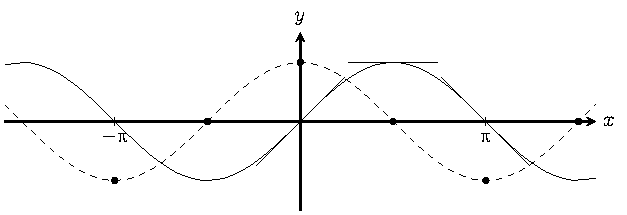
\includegraphics{basiccalculusandtrigonometry/sineandcosinerelation.pdf}
    \caption{The relation between sine (in black) and cosine (in dashed)}
    \label{fig:sine_cosine_relation}
\end{figure}

Let's start with the definition of the derivative given in \cref{eq:naive_definition_of_derivative},
\begin{equation}
    \odv*{\sin(x)}{x} = \lim_{h \appr 0}\frac{\sin(x + h) - \sin(x)}{h}.
\end{equation}
Using the sum of sines ($\sin(x + h) = \sin(x)\cos(h) + \cos(x)\sin(h)$),
\begin{align}
    \odv*{\sin(x)}{x} &= \lim_{h \appr 0}\frac{\sin(x)\cos(h) + \cos(x)\sin(h) - \sin(x)}{h}
    \intertext{When $h \appr 0$, $\cos(h) \appr 1$}
    &= \lim_{h \appr 0}\frac{\sin(x) + \cos(x)\sin(h) - \sin(x)}{h} \\
    &= \cos(x)\lim_{h \appr 0}\frac{\sin(h)}{h}.
    \intertext{For small angles, $\sin(h) \approx h$, therefore}
    &= \cos(x)\lim_{h \appr 0}\frac{h}{h} = \cos(x).
\end{align}
In conclusion, the derivative of sine is just the cosine just as we predicted with the graph.

Similarly, the derivative of cosine can also be found using the method of increments and using the sum of cosines formula $\cos(x + h) = \cos(x)\cos(h) - \sin(x)\sin(h)$
\begin{align}
	\odv*{\ab(\cos(x))}{x} &= \lim_{h \appr 0}\frac{\cos(x + h) - \cos(x)}{h} \\
						   &= \lim_{h \appr 0}\frac{\cos(x)\cos(h) - \sin(x)\sin(h) - \cos(x)}{h} \\
						   \intertext{When $h \appr 0$, $\cos(h) = 1$}
						   &= \lim_{h \appr 0}\frac{\cos(x) - \cos(x) - \sin(x)\sin(h)}{h} \\
						   &= \lim_{h \appr 0}\frac{-\sin(x)\sin(h)}{h}
						   \intertext{For small angles of $h$, $\sin(h) \approx h$}
						   &= \lim_{h \appr 0}\ab(-\sin(x)) = -\sin(x) 
\end{align}
I.e., the derivative of cosine is the negative of sine. From those two alone, we can form a set of formulas for differentiating sines and cosines:
\begin{equation}	
	\begin{aligned}
		\odv*{\ab(\sin(x))}{x} &= \cos(x) \\
		\odv*[order = 2]{\ab(\sin(x))}{x} &= \odv*{(\cos(x))}{x} = -\sin(x) \\
		\odv*[order = 3]{\ab(\sin(x))}{x} &= \odv*{(-\sin(x))}{x} = -\cos(x) \\
		\odv*[order = 4]{\ab(\sin(x))}{x} &= \odv*{(-\cos(x))}{x} = \sin(x)
	\end{aligned}
\end{equation}
We can see that the derivative of these two functions cycles in four: $\sin(x), \cos(x), -\sin(x), -\cos(x)$. From these alone, we can use the rules developed in \cref{sec:basic-derivatives-and-integrals}, e.g., the chain rule, power rule, etc., in order to find the derivative of other trigonometric functions.

\subsection{Derivative of other trigonometric functions}

Note that you can continue reading the next section straightaway. This section serves as a reference. But for those who are still interested, I'm glad to have you here. This is one of the places that uses the chain rule, product rule, and power rule a lot. It's a good exercise. Without further ado, let's start with the cosecant ($\csc(x) = \frac{1}{\sin(x)}$).
\begin{align}
	\odv*{\csc(x)}{x} &= \odv*{\frac{1}{\sin(x)}}{x} \\
						&= \odv*{\frac{1}{u}}{x} \cdot \odv{u}{u} && \textrm{Chain rule: $\sin(x) = u$} \\
						&= \odv*{u^{-1}}{u} \cdot \odv{u}{x} \\
						&= -1u^{-2}\cdot\odv*{\sin(x)}{x} && \textrm{Power rule, $u = \sin(x)$} \\
						&= -\frac{1}{\sin^2(x)}\cos(x) && \textrm{$\odv*{\sin(x)}{x} = \cos(x)$} \\
						&= -\csc(x)\cot(x) && \textrm{$\cot(x) = \frac{\cos(x)}{\sin(x)}$}.
\end{align}
And the secant function ($\sec(x) = \frac{1}{\cos(x)}$),
\begin{align}
	\odv*{\sec(x)}{x} &= \odv*{\ab(\frac{1}{\cos(x)})}{x} \\
					  &= \odv*{\ab(\frac{1}{u})}{x} \cdot \odv{u}{u} && \textrm{Chain rule: $\cos(x) = u$} \\
					  &= \odv*{u^{-1}}{u} \cdot \odv{u}{x} \\
					  &= -1u^{-2}\cdot\odv*{\cos(x)}{x} && \textrm{Power rule, $u = \cos(x)$}\\
					  &= -\frac{1}{\cos^{2}(x)}\ab(-\sin(x)) && \textrm{$\odv*{\cos(x)}{x} = -\sin(x)$} \\
					  &= \sec(x)\tan(x).
\end{align}

For the tangent function ($\tan(x) = \frac{\sin(x)}{\cos(x)}$), we use the product rule and the results from earlier
\begin{align}
	\odv*{\tan(x)}{x} &= \odv*{\frac{\sin(x)}{\cos(x)}}{x} \\
					  &= \odv*{\sin(x)\sec(x)}{x} \\
					  &= \sin(x)\odv*{\sec(x)}{x} + \sec(x)\odv*{\sin(x)}{x} \\
					  &= \sin(x)\sec(x)\tan(x) + \sec(x)\cos(x) \\
					  &= \sin(x)\frac{1}{\cos(x)}\frac{\sin(x)}{\cos(x)} + \frac{1}{\cos(x)}\cos(x) \\
					  &= \ab(\frac{\sin(x)}{\cos(x)})^2 + 1 = \tan^2(x) + 1 = \sec^2(x)
\end{align}
The Pythagorean identity is used in the last line to convert $1 + \tan^2(x)$ to $\sec^2(x)$. Of course, we cannot miss its reciprocal function: $\cot(x) = \frac{1}{\tan(x)}$.
\begin{align}
	\odv*{\cot(x)}{x} &= \odv*{\frac{1}{\tan(x)}}{x} \\
					  &= \odv*{\frac{\cos(x)}{\sin(x)}}{x} \\
					  &= \odv*{\cos(x)\csc(x)}{x} \\
					  &= \cos(x)\odv*{\csc(x)}{x} + \csc(x)\odv*{\cos(x)}{x} \\
					  &= \cos(x)\ab(-\csc(x)\cot(x)) + \csc(x)\ab(-\sin(x)) \\
					  &= -\cos(x)\frac{1}{\sin(x)}\frac{\cos(x)}{\sin(x)} - \frac{1}{\sin(x)}\sin(x) \\
					  &= -\ab(\cot^2(x) + 1) = -\csc^2(x),
\end{align}
where we've again used the Pythagorean identity $\cot^2(x) + 1 = -\csc^2(x)$.

Altogether, I've summarized all the derivatives of trigonometric functions into \cref{tab:derivative_trigonometric_functions}.
\begin{table}[ht]
	\begin{center}
		\begin{tabular}{C | L}
			f(x) & \odv*{f(x)}{x} \\
			\hline
			\sin(x) & \cos(x) \\
			\cos(x) & -\sin(x) \\
			\tan(x) & \sec^2(x) \\
			\hline
			\csc(x) & -\csc(x)\cot(x) \\
			\sec(x) & \sec(x)\tan(x) \\
			\cot(x) & -\csc^2(x)
		\end{tabular}
	\end{center}
	\caption{The derivatives of trigonometric functions}
	\label{tab:derivative_trigonometric_functions}
\end{table}

\section{Power series of trigonometric functions}

The approximation method that I'd be discussing are commonly taught to high schoolers with the name \textbf{small angle approximation}, i.e., for $\theta \appr 0$, \index{small angle approximation}
\begin{gather}
    \sin(\theta) \approx \tan(\theta) \approx \theta \mathand \cos(\theta) \approx 1 - \frac{\theta^2}{2}
\end{gather}
These approximations are very useful for calculating limits, e.g.,\footnote{Normally these limits are evaluated using the squeeze theorem. However, I don't want the mathematical intricacies to disrupt the flow of our journey right now. The full theorem will be discussed later at the end of the book.}
\begin{equation}
    \lim_{\theta \appr 0}\frac{\sin(n\theta)}{\theta} = \lim_{\theta \appr 0}\frac{n\theta}{\theta} = n.
\end{equation}
Here, I want to focus on where these approximations really comes from: the power series development of trigonometric functions.

\subsection{Power series of sine}

Assume that the sine function can be written as a power series
\begin{align}
	\sin(x) = s_0 + s_1x^1 + s_2x^2 + s_3x^3 + \dots
\end{align}
Because $\sin(0) = 0$,
\begin{align}
	\sin(0) &= s_0 + s_1(0)^1 + s_2(0)^2 + s_3(0)^3 + \dots \\
	s_0 = 0;
\end{align}
Because sine is an odd function, $\sin(-x) = -\sin(x)$; thus,
\begin{align}
	\begin{multlined}[b]
		s_1(-x)^1 + s_2(-x)^2 \\
		+ s_3(-x)^3 + s_4(-x)^4 + \dots
	\end{multlined} &=
	\begin{multlined}[t]
		-s_1x^1 - s_2x^2 \\
		- s_3x^3 - s_4x^4 + \dots 
	\end{multlined} \\
	\begin{multlined}[b]
		-s_1x^1 + s_2x^2 \\
		- s_3x^3 + s_4x^4 - \dots
	\end{multlined} &=
	\begin{multlined}[t]
		-s_1x^1 - s_2x^2 - \\
		s_3x^3 - s_4x^4 - \dots
	\end{multlined}
\end{align}
In the L.H.S., the sign alternates between negative and positive. In order for the L.H.S. to match the R.H.S., all the positive terms must vanish, leaving only the matching negative terms; therefore,
\begin{equation}
	\sin(x) = s_1x^1 + s_3x^3 + s_5x^5 + \dots.
\end{equation}
This is what we mean by \enquote{sine is an odd function}: there are only odd powers in its power series.

To find $s_1$, take the derivative of sine
\begin{equation}
	\odv*{\sin(x)}{x} = \cos(x) = s_1 + 3s_3x^2 + 5s_5x^4 + \dots,
\end{equation}
then substitute $x = 0$
\begin{align}
	\cos(0) = 1 &= s_1 + 3s_3(0)^2 + 5s_5(0)^4 + \dots \\
	1 &= s_1.
\end{align}
We can then take the derivative of sine again to get a recurrence relation.
\begin{align}
	\odv*[order = 2]{\sin(x)}{x} &= 3\cdot 2s_3x + 5\cdot 4s_5x^3 + 7\cdot 6s_7x^5 + \dots \\
	-\sin(x) &= \frac{3!}{1!}s_3x + \frac{5!}{3!}s_5x^3 + \frac{7!}{5!}s_7x^5 + \dots \\
	-s_1x - s_3x^3 - s_5x_5 - \dots &= \frac{3!}{1!}s_3x + \frac{5!}{3!}s_5x^3 + \frac{7!}{5!}s_7x^5 + \dots
\end{align}
By matching terms with the same order,
\begin{equation}	
	\begin{aligned}
		-s_1 &= \frac{3!}{1!}s_3x, \\
		-s_3 &= \frac{5!}{3!}s_5x, \\
		-s_5 &= \frac{7!}{5!}s_7x. \\
			 &\vdots
	\end{aligned}
\end{equation}
From $s_1 = 1$, we get that $s_3 = -\frac{1}{3!}$, $s_5 = -\frac{1}{5!}$, $s_7 = -\frac{1}{7!}$ etc. The negative sign alternates every term. We can then summarize the whole thing as
\begin{align}
	\sin(x) &= \sum_{n = 0}^{\infty}\frac{(-1)^{2n + 1}}{(2n + 1)!}x^{2n + 1} \\
			&= x - \frac{1}{3!}x^3 + \frac{1}{5!}x^5 - \frac{1}{7!}x^7 + \dots, \label{eq:sine-power-series}
\end{align}
which is the polynomial expansion of the sine function.

\subsection{Power series of cosine}

The power series of cosine can be developed using the same method as discussed earlier. But notice that the derivative of sine is cosine. Hence, we can just take the derivative of the sine's power series once to get the cosine's power series.
\begin{align}
	\odv*{\sin(x)}{x} &= \odv*{\ab(x - \frac{1}{3!}x^3 + \frac{1}{5!}x^5 - \frac{1}{7!}x^7)}{x} \\
	\cos(x) &= 1 - \frac{1}{2!}x^2 + \frac{1}{4!}x^4 - \frac{1}{6!}x^6 + \dots = \sum_{n = 0}^{\infty}\frac{(-1)^{2n}}{(2n)!}x^{2n}\label{eq:cosine-power-series}
\end{align}

\subsection{Power series of other trigonometric functions}

The same method could be used to find the power series expansion of secant, cosecant, tangent, etc. However, their power series doesn't actually represent the function because the other functions are all ratios of sine and cosines. To see what I mean, consider the behavior of the tangent function.

The tangent function is defined as $\tan\theta = \frac{\sin\theta}{\cos\theta}$. From this definition, $\tan\theta$ approaches infinity whenever $\cos\theta$ approaches zero, which is at $n\cpi$ where $n \in \mathbb{Z}$\footnote{$\mathbb{Z}$ is the set of integers}. As seen, there are infinitely many places in which the function approaches infinity. However, polynomials only have two infinities: at $x \appr \infty$, and $x \appr -\infty$; therefore, any polynomial expansion can't possibly represent the tangent function. The same logic also works for other trigonometric functions.

\subsection{Approximation of trigonometric functions}

One way a function can be approximated is by truncating its power series. To see why this is viable, consider the limit
\begin{align}
	\lim_{x \appr 0}\sin(x) = \lim_{x \appr 0}\ab(x - \frac{1}{3!}x^3 + \frac{1}{5!}x^5 - \frac{1}{7!}x^7 + \dots)
\end{align}
When $x \appr 0$, all the higher order degrees term vanishes; thus, 
\begin{gather}
	\lim_{x \appr 0}\sin(x) = x.
\end{gather}
It tells us that when $x \approx 0$, the sine function behaves like a linear function. Illustrated in \cref{fig:sine_small_angle},

\begin{figure}[ht]
	\centering
	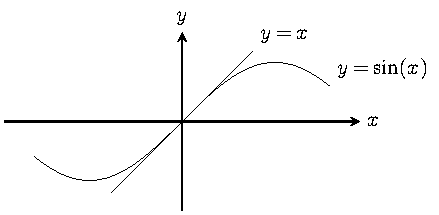
\includegraphics{basiccalculusandtrigonometry/sinesmallangle.pdf}
	\caption{Comparison of $y = \sin(x)$ and $y = x$ near $x = 0$}
	\label{fig:sine_small_angle}
\end{figure}
When $x$ gets larger, the higher order terms in the power series contributes more and more, so we need to include them. An excellent approximation for the sine function when $x \in [-\cpi, \cpi]$ is a truncation at the fifth term:
\begin{equation}
	\sin(x) \approx x - \frac{1}{3!}x^3 + \frac{1}{5!}x^5 - \frac{1}{7!}x^7 + \frac{1}{9!}x^9,
\end{equation}
plotted in \cref{fig:sine_approximation}. It is extremely accurate in that range.
\begin{figure}[t]
	\centering
	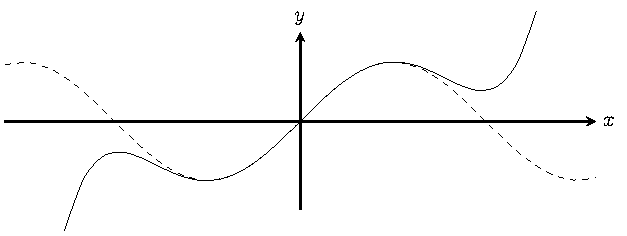
\includegraphics{basiccalculusandtrigonometry/sineapprox.pdf}
	\caption{An approximation of sine by truncating its power series at the fifth term.}
	\label{fig:sine_approximation}
\end{figure}
\begin{figure}[t]
	\centering
	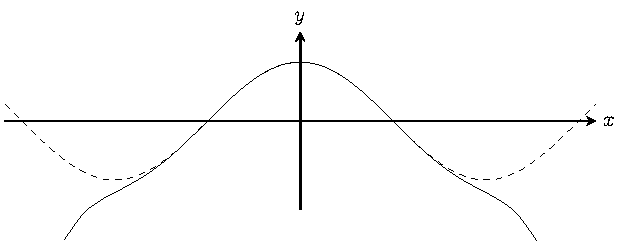
\includegraphics{basiccalculusandtrigonometry/cosineapprox.pdf}
	\caption{An approximation of cosine by truncating its power series at the fourth term}
	\label{fig:cosine_approximation}
\end{figure}
For cosine,
\begin{align}
	\lim_{x \appr 0}\cos(x) = \lim_{x \appr 0}\ab(1 - \frac{x^2}{2!} + \frac{x^4}{4!} - \dots) \approx 1 - \frac{x^2}{2!} \approx 1.
\end{align}
An acceptable approximation around zero is $1$ or $1 - \frac{x^2}{2}$. Similarly, an excellent approximation when $x \in [-\cpi, \cpi]$ is also a truncation at the fourth term:
\begin{equation}
	\cos(x) \approx 1 - \frac{1}{2!}x^2 + \frac{1}{4!}x^4 - \frac{1}{6!}x^6 
\end{equation}
plotted in \cref{fig:cosine_approximation}

\section{The harmonic oscillator}

\begin{figure}[ht]
	\centering
	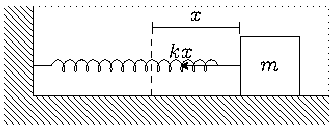
\includegraphics{basiccalculusandtrigonometry/harmonicoscillatorsetup.pdf}
	\caption{Setup of the harmonic oscillator}
	\label{fig:harmonic-oscillator-setup}
\end{figure}

Finally, we're ready to tackle our first oscillatory system: the harmonic oscillator. Illustrated in \cref{fig:harmonic-oscillator-setup}, consider a mass $m$ connected to a spring. The point that the spring is neither stretched or compressed is called the \textbf{equilibrium position}, drawn as the dashed line. The force that the spring acts on the mass depends on the displacement from the equilibrium position $x$:
\begin{equation}
	F = -kx,
\end{equation}
where $k$ is the stiffness of the spring. Higher $k$ represents a stiffer spring, and lower $k$ represents a looser spring. Newton's second law reads
\begin{align}
	-kx &= m\odv[ord = 2]{x}{t} \\
	-\frac{k}{m}x &= \odv[ord = 2]{x}{t}. \label{eq:spring-ord2}
\end{align}

We're interested in the solution of \cref{eq:spring-ord2} given an initial condition that at time $t = 0$, the mass is distance $A$ away from the equilibrium position, and it's released with zero initial velocity, i.e.,
\begin{equation}
	x(t = 0) = A \mathand \dot{x}(t = 0) = 0. \label{eq:spring-initial-condition}
\end{equation}

\subsection{Your first trigonometric substitution}

The equation that we got, \cref{eq:spring-ord2}, is an inseparable second order differential equation. It is extremely hard to work with. But by exploiting the chain rule, we can reduce it into a first order differential equation.
\begin{equation}
	\odv[ord = 2]{x}{t} = \odv*{\ab(\odv{x}{t})}{t} = \odv{\dot{x}}{t} = \odv{\dot{x}}{x}\odv{x}{t} = \dot{x}\odv{\dot{x}}{x}.
\end{equation}
\Cref{eq:spring-ord2} then becomes
\begin{align}
	-\frac{k}{m}x &= \dot{x}\odv{\dot{x}}{x} \\
	-\frac{k}{m}x\odif{x} &= \dot{x}\odif{\dot{x}} \\
	-\frac{k}{m}\int x\odif{x} &= \int\dot{x}\odif{\dot{x}} \\
	-\frac{k}{m}\frac{x^2}{2} &= \frac{\dot{x}^2}{2} + C \\
	-\frac{k}{m}x^2 &= \dot{x}^2 + C.
\end{align}
To find $C$, substitute in the initial condition \cref{eq:spring-initial-condition}.
\begin{align}
	-\frac{k}{m}(A)^2 &= (0)^2 + C \\
	C &= -\frac{k}{m}A^2. 
\end{align}
Thus,
\begin{align}
	-\frac{k}{m}x^2 &= \dot{x}^2 - \frac{k}{m}A^2 \\
	\dot{x}^2 &= \frac{k}{m}\ab(A^2 - x^2) \\
	\dot{x} &= \sqrt{\frac{k}{m}}\sqrt{A^2 - x^2}.
\end{align}
Because I'm too lazy to write square roots, let's use $\omega = \sqrt{\flatfrac{k}{m}}$; thus,
\begin{align}
	\dot{x} &= \omega\sqrt{A^2 - x^2} \\
	\odv{x}{t} &= \omega\sqrt{A^2 - x^2} \\
	\omega\odif{t} &= \frac{1}{\sqrt{A^2 - x^2}}\odif{x} \\
	\omega\int\odif{t} &= \int\frac{1}{\sqrt{A^2 - x^2}}\odif{x}. \label{eq:spring-ord1-d}
\end{align}
The L.H.S. directly evaluates to $\omega t$. But on the R.H.S., power rule substitution wouldn't work because there's a polynomial with degree two the root, but no terms with lower degree outside. If $u = A^2 - x^2$, we'd be going in loops. So how do we evaluate this?

The answer is, you can't do anything about it if we're going to use the methods so far. It's time for a new tool: \textbf{trigonometric substitution}.

The idea is very simple. We want to take advantage of the Pythagorean identity $1 - \sin^2\theta = \cos^2\theta$ to bring $A^2 - x^2$ out of the root. Substitute in $x = A\sin\theta$ and see what happens.
\begin{align}
	\int\frac{1}{\sqrt{A^2 - x^2}}\odif{x} &= \int\frac{1}{\sqrt{A^2 - A^2\sin^2\theta}}\odif{x} \\
										   &= \frac{1}{A}\int\frac{1}{\sqrt{1 - \sin^2\theta}}\odif{x} \\
										   &= \frac{1}{A}\int\frac{1}{\sqrt{\cos^2\theta}}\odif{x} = \frac{1}{A}\int\frac{1}{\cos\theta}\odif{x}
\end{align}
Taking care of the $\odif{x}$; if $x = A\sin\theta$, then
\begin{align}
	\odv{x}{\theta} &= A\odv{\sin\theta}{\theta} \\
	\odv{x}{\theta} &= A\cos\theta \\
	\odif{x} &= A\cos\theta\odif{\theta}.
\end{align}
Substituting back into the integral gives
\begin{equation}
	\frac{1}{A}\int\frac{1}{\cos\theta}\ab(A\cos\theta\odif{\theta}) = \int\odif{\theta} = \theta + C.
\end{equation}
Because $x = A\sin\theta$, $\theta = \arcsin\ab(\flatfrac{x}{A})$
\begin{equation}
	\int\frac{1}{\sqrt{A^2 - x^2}}\odif{x} = \arcsin\ab(\frac{x}{A}) + C.
\end{equation}
Thus, \cref{eq:spring-ord1-d} becomes
\begin{equation}
	\omega t = \arcsin\ab(\frac{x}{A}) + C.
\end{equation}
Then, substitute in the initial condition (\cref{eq:spring-initial-condition}) to find $C$:
\begin{align}
	\omega(0) &= \arcsin\ab(\frac{A}{A}) + C \\
	C &= \frac{\cpi}{2}.
\end{align}
Thus,
\begin{align}
	\omega t &= \arcsin\ab(\frac{x}{A}) + \frac{\cpi}{2} \\
	\arcsin\ab(\frac{x}{A}) &= \omega t + \frac{\cpi}{2} \\
	x &= A\sin\ab(\omega t + \frac{\cpi}{2}).
\end{align}
Since $\sin(\theta + \frac{\cpi}{2}) = \cos(\theta)$,
\begin{equation}
	x(t) = A\cos(\omega t) \label{eq:harmonic-oscillator-solution}
\end{equation}
which is the solution of the differential equation. It represents where the mass is relative to the equilibrium point over time. Taking the derivative of this once,
\begin{align}
	\dot{x}(t) &= A\odv{\cos(\omega t)}{t} \\
	\intertext{Let $u = \omega t$. By the chain rule,}
			&= A\odv{\cos(u)}{u} \times \odv{u}{t} \\
			&= -A\sin(u) \odv*{(\omega t)}{t} \\
			&= -\omega A\sin(\omega t), \label{eq:harmonic-oscillator-velocity}
\end{align}
we get the velocity as a function w.r.t. time. In a similar manner, taking the derivative of velocity again gives the acceleration
\begin{equation}
	\ddot{x} = \odv{\dot{x}}{t} = \odv{-A\omega\sin(\omega t)}{t} = -\omega^2A\sin(\omega t). \label{eq:harmonic-oscillator-acceleration}
\end{equation}

\subsection{The power series method}

Perhaps a faster method to solve \cref{eq:spring-ord2} is to just assume that the solution can be expanded in terms of power series
\begin{equation}
	x(t) = a_0 + a_1t + a_2t^2 + a_3t^3 + \dots. \label{eq:spring-series-x}
\end{equation}
Consequently,
\begin{gather}
	\dot{x}(t) = a_1 + 2a_2t + 3a_3t^2 + 4a^4t_3 + \dots \label{eq:spring-series-dot} \\
	\ddot{x}(t) = 2a_2 + 3\cdot 2a_3t + 4\cdot 3a_4t^2 + 5\cdot 4a_5t_3 + \dots \label{eq:spring-series-ddot}
\end{gather}
The initial condition given in \cref{eq:spring-initial-condition} ($x(t = 0) = A$, $\dot{x}(t = 0) = 0$) can then be used to find $a_0$ and $a_1$.
\begin{align}
	x(t = 0) &= a_0 + a_1(0) + a_2(0)^2 + a_3(0)^3 + \dots \\
	a_0 &= A
\end{align}
and from \cref{eq:spring-series-dot},
\begin{align}
	\dot{x}(t = 0) &= a_1 + 2a_2(0) + 3a_3(0)^2 + 4a_4(0)^3 + \dots \\
	a_1 &= 0
\end{align}
The rest of the terms can be found by using the differential equation itself. First, rearrange the equation into
\begin{equation}
	\odv[ord = 2]{x}{t} + \omega^2x = 0.
\end{equation}
Then, substitute in \cref{eq:spring-series-x,eq:spring-series-ddot}
\begin{align}
	0 &= \odv[ord = 2]{x}{t} + \omega^2x\\
	0 &= \begin{multlined}[t]
		\ab(2a_2 + 3\cdot 2a_3t + 4\cdot 3a_4t^2 + 5\cdot 4a_5t^3 + 6\cdot 5a_6t^4 + 6\cdot 7a_7t^5 + \dots) \\ + \ab(\omega^2A + a_2\omega^2t^2 + a_3\omega^2t^3 + a_4\omega^2t^4 + a_5\omega^2t^5\dots) \nonumber
	\end{multlined} \\
	0 &= \begin{aligned}[t]
		&\ab(2a_2 + \omega^2A) \\
		& +(3 \cdot 2a_3)t \\
		& +(4\cdot 3a_4 + \omega^2a_2)t^2 \\
		& +(5\cdot 4a_5 + \omega^2a_3)t^3 \\
		& +(6\cdot 5a_6 + \omega^2a_4)t^4 \\
		& +(7\cdot 6a_7 + \omega^2a_5)t^5 + \dots\\
	\end{aligned}
\end{align}
For the R.H.S. to be $0$, all terms must vanish; thus, we get an infinite series of equations to be evaluated
\begin{equation}
	\begin{aligned}
		0 &= \ab(2a_2 + \omega^2A) \\
		0 &= (3 \cdot 2a_3) \\
		0 &= (4\cdot 3a_4 + \omega^2a_2) \\
		0 &= (5\cdot 4a_5 + \omega^2a_3) \\
		0 &= (6\cdot 5a_6 + \omega^2a_4) \\
		0 &= (7\cdot 6a_7 + \omega^2a_5) \\
		  &\vdots
	\end{aligned}
\end{equation}
Starting from the second one: $0 = 3 \cdot 2a_3$ means that $a_3 = 0$. This eliminates every term that includes $a_3$. The fourth equation says $5\cdot 4a_5 + \omega^2a_3 = 0$, thus $a_5 = 0$. This pattern continues, eliminating every odd terms in the series. We're then left with
\begin{equation}
	\begin{aligned}
		0 &= 2a_2 + \omega^2A \\
		0 &= 4\cdot 3a_4 + \omega^2a_2 \\
		0 &= 6\cdot 5a_6 + \omega^2a_4 \\
		0 &= 8\cdot 7a_8 + \omega^2a_6 \\
		  &\vdots
	\end{aligned}
\end{equation}
Starting from the first one, we get $a_2 = -\frac{\omega^2}{2}A$. The second equation gives $a_4 = \frac{\omega^4}{4!}A$. The third gives $a_6 = \frac{\omega^6}{6!}A$. This pattern of $a_{2n} = \frac{\omega^{2n}}{2n}A$ continues on forever. The power series expansion for $x(t)$ gives
\begin{align}
	x(t) &= a_0 + \cancelto{0}{a_1} + a_2t^2 + \cancelto{0}{a_3}t^3 + a_4t^4 + \cancelto{0}{a_5}t^5 + a_6t^6 + \dots \\
		 &= A + A\frac{\omega^{2}}{2!}t^2 + A\frac{\omega^{4}}{4!}t^4 + A\frac{\omega^{6}}{6!}t^6 + \dots \\
		 &= A\ab(\frac{(\omega t)^2}{2!} + \frac{(\omega t)^4}{4!} + \frac{(\omega t)^6}{6!} + \dots)
\end{align}
Looks familiar yet? \emph{This}, the result that we got is exactly the power series expansion for cosine (\cref{eq:cosine-power-series}); thus,
\begin{equation}
	x(t) = A\cos(\omega t).
\end{equation}

\subsection{Physical aspects of the harmonic oscillator}

Now that we have solved the harmonic oscillator, let's bring our attention to the qualitative description of the system.

The mass is released with zero velocity at $x = A$. As the spring tries to restore its equilibrium, it accelerates the mass towards the equilibrium position. The further the mass is from the equilibrium, the stronger the spring pulls. Initially, the spring pulls very hard on the mass, causing it to accumulate much velocity. But as it approaches the equilibrium position, the spring's force diminishes and there is barely any force left to stop the mass, so it overshoots the other side, compressing the spring. This oscillatory cycle continues on forever. Intuitively, we can predict that the mass will have the highest velocity and lowest acceleration as it directly passes through the equilibrium; and, lowest velocity and highest acceleration when the spring is fully stretched or compressed. But does the mathematics agree with this?

In \cref{fig:harmonic-oscillator-position-velocity}, the position function (\cref{eq:harmonic-oscillator-solution}) is plotted in thick lines, and the velocity function (\cref{eq:harmonic-oscillator-velocity}) are plotted in dashed lines.

The furthest point that a mass could be from a spring is at $x = \pm A$. Mathematically, this represents the local maxima and minima of the function, which can be obtained by taking the first derivative and setting it to zero (\cref{sec:minima-and-maxima}). The derivative of the position w.r.t. time is just the velocity (\cref{eq:harmonic-oscillator-velocity}), and it reaches zero whenever $\sin(\omega t)$ is zero
\begin{align}
	\sin(\omega t) &= 0 \\
	\omega t &= \arcsin(0) + 2n\cpi && n \in \mathbb{Z}\\
	t &= \frac{(2n + 1)\cpi}{\omega}. \label{eq:harmonic-oscillator-max-position}
\end{align}
Another way to derive this fact is to just notice that the range of the cosine function only extends from $-1$ to $1$; therefore, the highest that $A\cos(\omega t)$ can go is just $A$. So, another equation that we can form is
\begin{align}
	\cos(\omega t) = 1 \\
	\omega t = \arccos(1) + 2n\cpi && n \in \mathbb{Z} \\
	t = \frac{(2n + 1)\cpi}{\omega},
\end{align}
which has the same solution as $\sin(\omega t) = 0$.

\begin{figure}[ht]
	\centering
	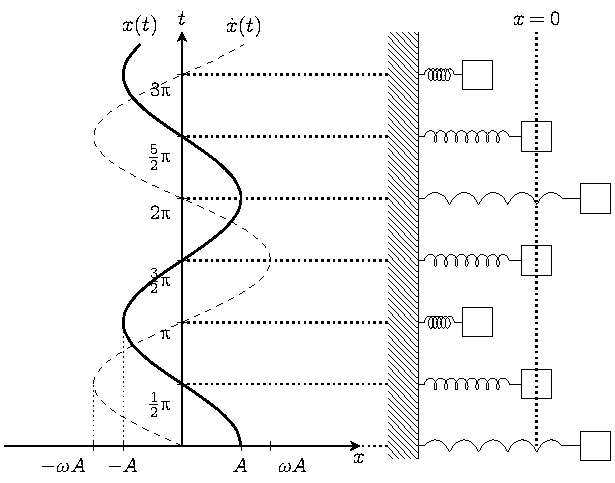
\includegraphics{basiccalculusandtrigonometry/harmonic-oscillator-position-velocity.pdf}
	\caption{The trajectory of a mass in the harmonic oscillator system. (Left) The position is plotted in thick lines, and the velocity, in dotted lines. (Right) Depiction of an oscillating mass, according to the solution of the differential equation.}
	\label{fig:harmonic-oscillator-position-velocity}
\end{figure}

The time that the mass goes through the equilibrium position can be found by just setting $A\cos(\omega t)$ to zero
\begin{align}
	A\cos(\omega t) &= 0 \\
	\omega t &= \arccos(0) + 2n\cpi && n \in \mathbb{Z}\\
	t &= \frac{2n\cpi}{\omega} \label{eq:harmonic-oscillator-zero-position}
\end{align}

Since the velocity function (\cref{eq:harmonic-oscillator-velocity}) is a sine function, it must oscillates $\cpi$ radians off-phase relative to the position function. Therefore, 
\begin{enumerate}
	\item Whenever the mass is furthest away from the equilibrium, the velocity is zero
	\item Whenever the mass is directly passing through the equilibrium, the velocity reaches its maximum at $\pm\omega A$
\end{enumerate}
The first fact can be easily verified by setting the velocity function, $-\omega A\sin(\omega t)$ equals to zero
\begin{align}
	-\omega A\sin(\omega t) &= 0 \\
	\omega t &= \arcsin(0) + 2n\cpi \\
	t &= \frac{(2n + 1)}{\omega},
\end{align}
which directly matches with the point of furthest position (\cref{eq:harmonic-oscillator-max-position}). The second one can be verified by taking the derivative of velocity, which is just the acceleration, found in \cref{eq:harmonic-oscillator-acceleration}. Setting that equals to zero yields
\begin{align}
	-\omega^2A\cos(\omega t) &= 0 \\
	\omega t &= \arccos(0) + 2n\cpi \\
	t &= \frac{2n\cpi}{\omega},
\end{align}
which matches our result from \cref{eq:harmonic-oscillator-zero-position}.

The acceleration function is again, a cosine function that's in phase with the position. Therefore, the local minima and maxima from the position function must match. We can quickly conclude that the acceleration is at its highest at $t = \frac{2n\cpi}{\omega}$, and is zero at $\frac{(2n + 1)\cpi}{\omega}$.

You would think that we have completed the physical aspects of the harmonic oscillator. But there is something I left over: the $\omega$ term. Since the beginning, I have assigned $\omega = \sqrt{\frac{k}{m}}$ as a notational trick for convenience. Is there any real physical meaning behind $\omega$?

If you don't know much about units, it's fine if you skip these paragraphs straightaway. But one clue that suggests the physical meaning of $\omega$ is its unit. Since $\omega = \sqrt{\frac{k}{m}}$, we have to analyse the units of its components separately. $k$ is a spring stiffness constant which is got from
\begin{equation}
	F = -kx \mathor k = -\frac{F}{x}.
\end{equation}
$F$ is the unit of force (Newton $\unit{\newton}$), which is just $\unit{\kilogram}\frac{\unit{\meter}}{\unit{\second^2}}$), and $x$, the units of distance (Meters $\unit{\meter}$); therefore, $k$ is the unit of
\begin{equation}
	\frac{\unit{\kilogram}\frac{\unit{\meter}}{\unit{\second^2}}}{\unit{\meter}} = \frac{\unit{\kilogram}}{\unit{\second^2}}.
\end{equation}
And since $m$ has the unit of kilogram ($\unit{\kilogram}$), $\omega$ which is $\sqrt{\frac{k}{m}}$ has the unit of
\begin{equation}
	\sqrt{\frac{\frac{\unit{\kilogram}}{\unit{\second^2}}}{\unit{\kilogram}}} = \sqrt{\frac{1}{\unit{\second^2}}} = \frac{1}{\unit{\second}}
\end{equation}
Funnily enough, this is the unit of Hertz, ($\frac{1}{\unit{\second}} = \unit{\hertz}$) which describes a frequencies. But it cannot possibly be just a unit of frequency because the solution of the differential equation says so.

The solution of our equation is $x(t) = A\cos(\omega t)$. If $\omega$ is really a unit of Hertz, then $\omega t$ would have no units, which contradicts that the cosine function either accepts radians ($\unit{\radian}$), or degrees ($\unit{\deg}$). But these are units that are dimensionless, meaning that we can just multiply it into $\omega$; therefore, $\omega$ must have the unit of $\unit{\radian\per\second}$, which is the unit of angular frequencies.

The conclusion that $\omega$ is the angular frequencies can also be directly deducted from the solution of the equation. From both of \cref{eq:harmonic-oscillator-max-position} and \cref{eq:harmonic-oscillator-zero-position}, the time between each maximum and minima point is divided by $\omega$. If $\omega$ is very high, then the time between the maximum and minimum is decreased. If it's low, then the time is increased. Therefore, $\omega$ is directly associated to the natural frequency of the system. The more $\omega$ is, the more frequent the oscillator oscillates.

Another way $\omega$ can be interpretted is by looking at the expression of $\omega$ itself: $\sqrt{\frac{k}{m}}$. The spring stiffness constant $k$ is on the top, so it means the stiffer the spring, the higher omega is. A stiffer spring would allow the spring to pull the mass faster; thus, increasing the frequencies. The mass $m$ is on the bottom: the larger the mass, the lower the omega. That just means a more massive block is harder for the spring to move; therefore, the mass will travel slower, decreasing the frequencies.

\subsection{Solution for other initial conditions. A trick with simplifying inverse trigonometric functions.}

Now, let's see what happens if the initial condition is changed from $x(t = 0) = A$, and $v(t = 0) = 0$, to
\begin{equation}
	x(t = 0) = X \mathand v(t = 0) = V.
\end{equation}
Since it's the same system but just under a different initial condition, the differential equation stays exactly the same
\begin{equation}
	\odv[ord = 2]{x}{t} + \omega^2x = 0,
\end{equation}
where $\omega = \sqrt{\flatfrac{k}{m}}$ for the same notational reason. In a similar manner, use the chain rule on the second derivative to reduce it down to a first order differential equation:
\begin{align}
	\dot{x}\odv{\dot{x}}{x} &= -\omega^2x \\
	\dot{x}^2 &= -\omega^2x^2 + C.
\end{align}
To find the initial condition, set $t = 0$ and substitute $x(t = 0) = X$ and $v(t = 0) = V$.
\begin{align}
	V^2 &= -\omega^2(X)^2 + C \\
	C &= \omega^2X^2 + V^2.
\end{align}
Since the form is quite complex, let's call this $C_1$, and substitute it in later when the differential equation is fully solved. So,
\begin{align}
	\dot{x}^2 &= -\omega^2x^2 + C_1 \\
	\odv{x}{t} &= \sqrt{-\omega^2x^2 + C_1} \\
	\int\odif{t} &= \int\frac{1}{\sqrt{C_1 - \omega^2x^2}}\odif{x} \\
	t &= \int\frac{1}{\frac{1}{\omega}\sqrt{\ab(\flatfrac{\sqrt{C_1}}{\omega})^2 - x^2}}\odif{x} \\
	t &= \omega\int\frac{1}{\sqrt{\ab(\flatfrac{\sqrt{C_1}}{\omega})^2 - x^2}}\odif{x}
\end{align}
Since $C_1$ is always positive due to its term all being squared. The same trigonometric substitution can be used to obtain
\begin{align}
	t = \omega\arcsin\ab(\frac{x}{\flatfrac{\sqrt{C_1}}{\omega}}) + C_2
\end{align}
Then, set $t = 0$, and substitute $x(t = 0) = X$ to find $C_2$.
\begin{align}
	0 &= \omega\arcsin\ab(\frac{\omega X}{\sqrt{C_1}}) + C_2 \\
	C_2 &= -\omega\arcsin\ab(\frac{\omega X}{\sqrt{\omega^2X^2 + V^2}})
\end{align}


\subsection{The ansatz method}

\section{Damped harmonic oscillator}

\section{Substitution to eliminate trigonometric functions}

\section{Circles and ellipses}

\subsection{Perimeter}

\subsection{Areas of circle. A funny way to approximate pi.}

\section{Volume of revolutions}

\chapter{Merging calculus and dynamical systems}
\label{sec:calculus-and-physical-systems}

As said earlier, with the merge of calculus and trigonometry, all the cards are on the deck. This is all the calculus knowledge there is from here to the nineteenth-century.

\section{Further examples of calculus in physics and kinematics}

\subsection{Block sliding down a ramp with friction}

\begin{figure}[ht]
    \centering
    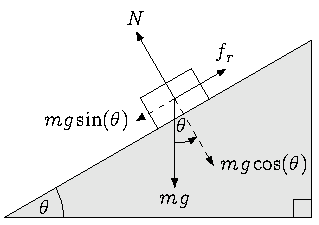
\includegraphics{geometricalsignificance/blockslidingdownaramp}
    \caption{A block sliding down a rough ramp (i.e. with friction) angled $\theta$ relative to the ground}
    \label{fig:blockslidingdownaramp}
\end{figure}
Illustrated in \cref{fig:blockslidingdownaramp}, there are two axis of motion: perpendicular and parallel to the block's expected motion. From what we know, there are the gravity $mg$ that pulls the block straight down and the friction force $f_r$ acting against the block's expected motion in the parallel axis. The problem constraints use along the perpendicular axis: the block can't move along that perpendicular axis \emph{because there's a ramp in the way}. Therefore, the ramp must act a force $N$ on the block.

We want to find the equation of motion for this block that's sliding down a ramp with friction. As far as the perpendicular axis goes, we don't have to worry about that one because nothing is moving there anyways. On the parallel axis, there's the $f_r$ and $mg\sin(\theta)$.\footnote{Just decompose $mg$ into its parallel and perpendicular axis. Using basic trigonometry is enough.} If we set the direction of the parallel axis to pointing downwards along the block's movement, we get that the total force is
\begin{equation*}
    F_{n} = mg\sin(\theta) - f_r\footnote{$F_n$ for $F_{\textrm{net}}$ or, total force.}.
\end{equation*}
By the Newton's second law,
\begin{align*}
    m\odv{t}(\odv{x}{t}) = mg\sin(\theta) - f_r \\
    \odv{t}(\odv{x}{t}) = g\sin(\theta) - \frac{f_r}{m}.
\end{align*}
$g\sin(\theta) - \flatfrac{f_r}{m}$ doesn't change with time, let's name it $\kappa$. The equation then becomes
\begin{align}
    \odv{t}(\odv{x}{t}) &= \kappa \label{eq:blockslidingdownarampaux}\\
    \int\odif(\odv{x}{t}) &= \int\kappa\odif{t} \nonumber\\
    \odv{x}{t} &= \kappa t \nonumber \\
    \int\odif{x} &= \int\kappa t\odif{t} \nonumber\\
    x(t) &= \left(g\sin(\theta) - \frac{f_r}{m}\right)\frac{t^2}{2}.
\end{align}
which \emph{is} our equation of motion. Notice, \cref{eq:blockslidingdownarampaux} literally has the same form as \cref{eq:accelerationfromgravity} that we derived from ``ball dropped from a building''. And indeed, it should be the same because it's just a thing that's under a constant acceleration. 

\subsection{One-dimensional movement with drag forces}

The free body diagram is illustrated in \cref{fig:projectileswithdragforce}. There's the gravity $m\vv{g}$ pulling the ball down, and drag force $kf_r(\vv{v})$. However, drag is a complex thing. There is no such thing as an ``exact drag function'' because drag depends on so many variables, e.g., air viscosity, air compressibility, object's shape, surface's friction, just to name a few. Therefore, the drag function $f_r(\vv{v})$ is a \emph{simplified model}, not the real thing.\index{drag function (simplified model)}

We shall model the drag based on two assumptions. \begin{enumerate*}[label = \roman*.)]
    \item the drag force should depend on the velocity : the faster, the more drag. And,
    \item any function can be approximated using the power series expansion (also discussed in \cref{sec:afunctionthatisitsownderivative}):
\end{enumerate*}
\begin{equation*}
    f_r(\vv{v}) = a_0 + a_1\vv{v} + a_2\vv{v}^2 + a_3\vv{v}^3 + \dots.
\end{equation*}
Considering only the first three terms should be enough. We know that $a_0$ must be $0$, because otherwise our object would just accelerate all the time, which is no good. Therefore, there can only be $a_1\vv{v} + a_2\vv{v}^2$. Newton's second law reads
\begin{equation*}
	m\odv*{(\odv{x}{t})}{t} = a_1\odv{x}{t} + a_2\ab(\odv{x}{t})^2.
\end{equation*}
Using fluxion notation,
\begin{align*}
    m\odv{\dot{x}}{t} &= a_1\dot{x} + a_2\dot{x}^2 \\
    \odv{\dot{x}}{t} &= \frac{a_1}{m}\dot{x} + \frac{a_2}{m}\dot{x}^2
\end{align*}
For convenience, let $\flatfrac{a_1}{m} = p$ and $\flatfrac{a_2}{m} = q$. The equation reads
\begin{equation}
    \odv{\dot{x}}{t} = p\dot{x} + q\dot{x}^2. \label{eq:quadraticdrageq}
\end{equation}

It is obvious that both $p$ and $q$ must be negative, otherwise the object would accelerate forward with the velocity. Frankly, \cref{eq:quadraticdrageq} is not possible to solve using the techniques that we have now. I'll revisit this exact differential equation later in \cref{eq:advtechniquesrationalfunctions}. For now, we shall deal with a simpler equation by considering two cases: only linear drag and only quadratic drag.

\subsubsection{Motion with just linear drag}

You don't really see linear drag in real life. It's mostly drag in moving liquid, e.g., a fish swimming in the water. \Cref{eq:quadraticdrageq} simplifies to
\begin{equation*}
    \odv{\dot{x}}{t} = p\dot{x}.
\end{equation*}
I shall set $v_0$ as the initial velocity and $x_0$ as the initial position. There are two methods of solving this. First, by separating variables using analytical methods.
\begin{align}
    \int\frac{1}{\dot{x}}\odif{\dot{x}} &= p\int\odif{t} \nonumber\\
    \ln(\dot{x}) + C &= pt. \label{eq:motionlineardrag1}
\end{align}
To find out what this integration constant should be, we have to use the initial condition $t = 0 \implies \dot{x} = v_0$.
\begin{align*}
    \ln(v_0) + C &= 0 \\
    C &= -\ln(v_0).
\end{align*}
\Cref{eq:motionlineardrag1} then becomes
\begin{align}
    \ln(\dot{x}) - \ln(v_0) &= pt \nonumber\\
    \dot{x} &= v_0\e^{pt}. \label{eq:motionlineardrag2}
\end{align}

\begin{figure}
    \centering
    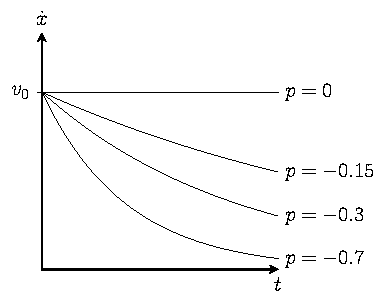
\includegraphics{geometricalsignificance/motionlineardragv}
    \caption{Plot of \cref{eq:motionlineardrag2} with various $p$.}
    \label{fig:motionlineardragv}
\end{figure}
\Cref{fig:motionlineardragv} plots \cref{eq:motionlineardrag2} with various $p$. Notice that when $p = 0$, \cref{eq:motionlineardrag2} is just a straight line $\dot{x} = v_0$. The more negative $p$ is, the faster it slows down, as illustrated. That is why sometimes, we call $p$ the \textbf{dampening factor}\index{dampening factor}. Also, $v_0$ here just scales the graph in the $\dot{x}$ direction.

To find $x(t)$, we rewrite \cref{eq:motionlineardrag2} as
\begin{equation*}
    \odv{x}{t} = v_0\e^{pt}.
\end{equation*}
Then,
\begin{align}
    \odif{x} &= v_0\e^{pt}\odif{t} \\
    x + C_1 &= v_0\int \e^{pt}\odif{t}. \label{eq:motionlineardrag3}
\end{align}

Here, I shall introduce an integration technique called \textbf{change of variables}\index{change of variables!naive}, commonly known as $u$-substitution. We'll formally come back to this topic later in \cref{sec:changeofvariables}. Basically, it's a way to convert integrals that we don't recognize into an easier integral. It's better if I just show the examples. We don't know the antiderivative of $\e^{pt}$ in \cref{eq:motionlineardrag3}, however we know the antiderivative of $\e^{u}$. So let's convert $\e^{pt}$ into that form. By letting a dummy variable $u = pt - v_0$, we have to convert $\odif{u}$ into $\odif{t}$ aswell.
\begin{align*}
    u &= pt - v_0 \\
	\odv{u}{t} &= \odv*{(pt - v_0)}{t} \\
    \frac{1}{p}\odif{u} &= \odif{t}.
\end{align*}
Then, substituting $\odif{t} = \frac{1}{p}\odif{u}$ and $u = pt$ into \cref{eq:motionlineardrag3}, it reads
\begin{align}
    x + C_1 &= v_0\int\e^{u}\ab(\frac{1}{p}\odif{u}) \nonumber\\
    x + C_1 &= \frac{v_0}{p}\e^{pt}. \label{eq:motionlineardrag4}
\end{align}

We also have to take care of the $C_1$. Using $t = 0 \implies x = x_0$,
\begin{align*}
    x_0 + C_1 &= \frac{v_0}{p}\e^{p\cdot(0)} \\
    C_1 &= \frac{v_0}{p} - x_0.
\end{align*}
Then, plug it into \cref{eq:motionlineardrag4}. The equation becomes
\begin{align}
    x + \frac{v_0}{p} - x_0 &= \frac{v_0}{p}(\e^{pt}) \nonumber\\
    x &= x_0 + \frac{v_0}{p}(\e^{pt} - 1). \label{eq:motionlineardrag5}
\end{align}

I've plotted \cref{eq:motionlineardrag5} with varying $v$ in \cref{fig:motionlineardragx1} and varying $p$ in \cref{fig:motionlineardragx2}. The graph should match with what you expect intuitively: higher $v$ will get you further, and the less the drag, the further you'll get.

\begin{figure}[ht]
    \centering
    \begin{subfigure}[l]{0.45\textwidth}
        \centering
        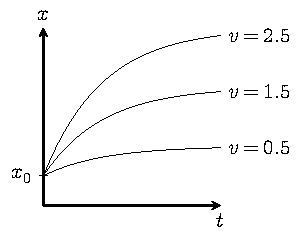
\includegraphics{geometricalsignificance/motionlineardragx1}
        \caption{with varying $v$, setting $p = -1$}
        \label{fig:motionlineardragx1}
    \end{subfigure}
    \begin{subfigure}[r]{0.45\textwidth}
        \centering
        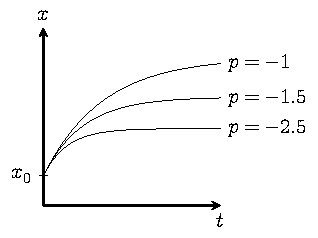
\includegraphics{geometricalsignificance/motionlineardragx2}
        \caption{with varying $p$, setting $v = 2$}
        \label{fig:motionlineardragx2}
    \end{subfigure}
    \caption{Plot of \cref{eq:motionlineardrag5}, setting $x_0 = 0.5$.}
\end{figure}

Notice, this motion has a clear upper limit. \emph{If $p \in \mathbb{R}^-$}, $\lim_{t \appr \infty}e^{pt} = 0$. Taking the limit as $t \appr 0$ on both sides of \cref{eq:motionlineardrag5}, we get
\begin{align*}
    \lim_{t \appr \infty} x(t) &= \lim_{t \appr \infty}\left(x_0 + \frac{v_0}{p}(e^{pt} - 1)\right). \\
    &= x_0 + \frac{v_0}{p}\cancelto{0}{\lim_{t \appr 0}\left(e^{pt}\right)} - \frac{v_0}{p} = x_0 - \frac{v_0}{p},
\end{align*}
which when $p \in \mathbb{R}^-$ and $v_0\in\mathbb{R}^+$, the motion procedes forward, then gradually slows down and stops at $x_0 - \frac{v_0}{p}$ which is more than $x_0$.

\subsubsection{Motion with just quadratic drag}

\begin{multicols}{2}
This equation is even easier than linear drag, so I'd leave out some steps. \Cref{eq:quadraticdrageq} simplifies to
\begin{align*}
    \odv{\dot{x}}{t} &= q\dot{x}^2 \\
    \int \frac{1}{\dot{x}^2}\odif{\dot{x}} &= q\int\odif{t} \footnote{Hint: $\flatfrac{1}{\dot{x}^2} = \dot{x}^{-2}$}\\
    - \frac{1}{\dot{x}} + C = qt.
\end{align*}
Taking care of $C$: use $t = 0 \implies \dot{x} = v_0$.
\begin{align*}
    - \frac{1}{v_0} + C &= q\cdot 0 \\
    C &= \frac{1}{v_0}.
\end{align*}
Therefore,
\begin{align}
    -\frac{1}{\dot{x}} + \frac{1}{v_0} &= qt \nonumber\\
    \odv{t}{x} &= \frac{1 - qv_0t}{v_0} \nonumber\\
    x &= v_0\int\frac{1}{1 - qv_0t} \odif{t}. \label{eq:motionquadraticdrag1}
\end{align}
The structure of the integral is similar to $\flatfrac{1}{t}$. Therefore, let $u = 1 - qv_0t$. Then,
\begin{align*}
    \odv{u}{u} &= \odif{u}(1 - qv_0t) \\
    1 &= -qv_0\odv{t}{u} \\
    \odif{t} &= -\frac{1}{qv_0}\odif{u}.
\end{align*}
Substitute $u = 1 - qv_0t$ and $\odif{t} = -\frac{1}{qv_0}\odif{u}$ into \cref{eq:motionquadraticdrag1}:
\begin{align}
    x &= v_0 \int \frac{1}{u}\left(-\frac{1}{qv_0}\odif{u}\right) \nonumber\\
    &= -\frac{1}{q}\int \frac{1}{u}\odif{u} \nonumber\\
    x(t) &= -\frac{1}{q}\ln(1 - qv_0t) + C_1. \label{eq:motionquadraticdrag2}
\end{align}
Taking care of $C_1$: use $t \appr 0 \implies x(t) = x_0$.
\begin{align*}
    x_0 &= -\frac{1}{q}\ln(1 - qv_0\cdot(0)) + C_1 \\
    x_0 &= C_1
\end{align*}
Plug this into \cref{eq:motionquadraticdrag2} to get the final answer:
\begin{equation*}
    x(t) = -\frac{1}{q}\ln(1 - qv_0t) + x_0.
\end{equation*}
\end{multicols}

Surprisingly, quadratic drag does not have upper position bounds. A bit more thought would reveal that when $v < 0$, the quadratic drag $f_r(v) = a_2v^2$ is smaller thasecn $f_r(v) = a_1v$. Thus, it should makes sense that quadratic doesn't have bounds, but linear has an upper bound.

\subsubsection{Terminal velocity of objects}

\subsection{Time of meteor collision from great height}

Illustrated in \cref{fig:meteorfallingfromgreatheight}\footnote{Not to scale.}, a meteor is falling from height $h$ above the Earth. Let's find the time that it'd take to hit the Earth.
\begin{figure}[ht]
    \centering
    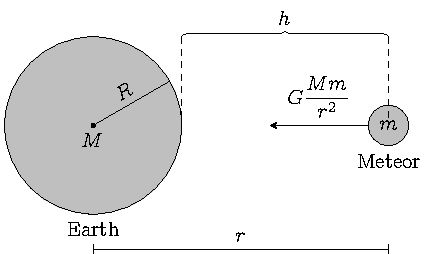
\includegraphics{geometricalsignificance/meteorfallingfromgreatheight}
    \caption{An illustration of a meteor falling to the Earth from height $h$.}
    \label{fig:meteorfallingfromgreatheight}
\end{figure}
The meteor has the mass $m$, falling from height $h$ above the ground. The Earth has mass $M$, radius $R$. Let's denote the meteor's position relative to the Earth's center with $r$. The initial condition of the meteor is $r(0) = h + R$, and $\dot{r}(0) = v_0$ For simplicity sake, let the meteor be a mass point: its radius is zero, and the Earth is very massive compared to the meteor so it doesn't move with the meteor's gravitational attraction. Given by Newton's law of gravitational attraction, the Earth is pulling the meteor by
\begin{equation*}
    F = G\frac{Mm}{r^2}.
\end{equation*}
Therefore, Newton's second law on the meteor reads
\begin{equation*}
	G\frac{Mm}{r^2} = m\odv*{\ab(\odv{r}{t})}{t}\footnote{Notice that here, $r$ also changes with time.}.
\end{equation*}

To frame the problem mathematically, we want to find an equation of motion of the meteor. Then, find the time it takes for the meteor to travel from $h + R$ (initial position) to $R$ (the ground).

The $m$ on both sides cancel. For convenience, let $\kappa = GM$
\begin{equation}
    \frac{\kappa}{r^2} = \odv{\dot{r}}{t}. \label{eq:meteorfallingfromgreatheight1}
\end{equation}
Solving this equation is not at all trivial: there are \emph{three} variables, i.e., $r$. $\dot{r}$, and $t$; however, an equation only has two sides. We can't possibly separate these variables. Here, I shall introduce a technique for solving this kind of differential equation. With the chain rule,
\begin{equation*}
    \odv{\dot{r}}{t} = \odv{\dot{r}}{r} \cdot \odv{r}{t} = \dot{r}\odv{\dot{r}}{r}:
\end{equation*}
we converted an expression that's dependent on other variable $t$ to be dependent on a lower derivative $r$ instead! Then $t$ is removed, or rather, hidden. You can interpret $\odv*{\dot{r}}{r}$ as the velocity at any given distance away from the Earth. Plug this into \cref{eq:meteorfallingfromgreatheight1}, we get
\begin{align}
    \frac{\kappa}{r^2} &= \dot{r}\odv{\dot{r}}{r} \nonumber\\
    \kappa\int\frac{1}{r^2}\odif{r} &= \int\dot{r}\odif{\dot{r}} \nonumber\\
    \frac{\kappa}{r} + C &= \frac{\dot{r}^2}{2} \label{eq:meteorfallingfromgreatheight2}
\end{align}
The term $+C$ is going to be a different because now, we don't have a $t$ to fix our initial condition. However, we know that when $\dot{r} = v_0$, $r = h + R$. Therefore,
\begin{align*}
    -\frac{\kappa}{h + R} + C &= \frac{v_0^2}{2} \\
    C &= \frac{v_0^2}{2} - \frac{\kappa}{r}.
\end{align*}
However, the structure of $C$ is quite complicated so, I wouldn't substitute it in yet until we get our final answer. Continuing with \cref{eq:meteorfallingfromgreatheight2}, we turn the $\dot{r}$ into the Leibniz's notation:
\begin{align*}
    \frac{\kappa + Cr}{r} &= \frac{1}{2}\left(\odv{r}{t}\right)^2. \\
    \sqrt{2}\sqrt{\frac{\kappa + Cr}{r}} &= \odv{r}{t} \\
    \int\odif{t} &= \sqrt{2}\int\sqrt{\frac{r}{\kappa + Cr}}\odif{r}
\end{align*}

Unfortunately, this integral is very hard to solve. But it is possible, and the solution to this integral is
\begin{equation*}
    \frac{C}{\kappa^{\flatfrac{3}{2}}\sqrt{r}}\sqrt{\frac{r}{\kappa r + C}}\sqrt{\frac{\kappa r}{C} + 1} \left(\sqrt{\kappa r}\sqrt{\frac{\kappa r}{C} + 1} - \sqrt{C}\sinh^{-1}\left(\sqrt{\frac{\kappa x}{C}}\right)\right),
\end{equation*}
which is quite a nightmare, but we will get back to this in the far far future.

\subsection{Damped harmonic motion}

\section{Conservation laws}

% \chapter{Series}

\section{Sequences}

\section{Geometric series: zeno's paradox}

\section{Convergence and divergence}

\subsection{Absolute convergence}

\section{Convergence test}

\section{Harmonic motion: the need of functions approximation}

\section{Taylor series}

\part{Signal analysis}

% \chapter{Basic techniques of integration}
\label{sec:techniquesofintegration}

\begin{abstract}
    This chapter explores various techniques you can use to integrate stuffs. You still have to keep in mind that even though this chapter is very abstracted away, \emph{integrals still have its geometric meaning: area under the graph.} This geometric interpretation is going to somewhat appear quite often throughout the chapter, so be aware of it.

    Also, some integrals are definite: they have clear boundaries of integrations. You also have to keep track of what variable is bounded by that bound, otherwise you might end up evaluating incorrectly.
\end{abstract}

Note from the writer: As a calculus teacher myself, I usually don't teach this topic but leave it as an exercise. Techniques of integrations come naturally with much experiences. Therefore, I list a table of integrations at the end of the chapter for the physicists out there.

\section{Change of variables}
\label{sec:changeofvariables}

Change of variables, or integration by substitution is a method to convert an unknown integrals into a more familiar one. Consider $\int x\e^(x^2)\dd{x}$. This integral might seem daunting at first but, notice that the derivative of $x^2$ is exactly $x$. I shall introduce a new variable $u$ where $u = x^2$. If we take the derivative w.r.t. $x$ on both sides,
\begin{align*}
    \dv{u}{x} = 2x \\
    \dv{u} = 2x\dd{x}.
\end{align*}

\section{Integrals of inverse functions}

\section{Integrals of symmetric functions}

\subsection{Even and odd functions}

\subsection{Functions with axial and spherical symmetry}

\section{Integration by part}

\section{Recurrence relations and reduction formulas}

\section{Working with complex numbers and exponentials}

\section{Trigonometric substitution}

\section{Rational functions}

\subsection{Partial fraction decomposition}

\subsection{Quadratic under radicals}

\subsection{Ostrogradski method}

\section{Feynman's trick for integration}

\section{Polar integration}

\section{Gaussian integral}

\section{Cauchy's formula for repeated integrations}

\section{Numerical integration}
% \chapter{Advanced techniques of integration}
\label{sec:advancedtechniquesofintegration}

\begin{abstract}
    This is the chapter that explores more advanced techniques of integrations. You could go on with your life skipping this chapter and it'd still be fine. However, for the curious, there are some very interesting maths in here, so be sure to check this chapter out before going on to the next part of the book.
\end{abstract}

\section{Rational functions}
\label{eq:advtechniquesrationalfunctions}

\subsection{Quadratics denominator}

An integral in the form
\begin{equation}
    \int \frac{1}{ax^2 + bx + c}\dd{x}
\end{equation}
can be evaluated by completing the squares:
\begin{equation}
    ax^2 + bx + c = a\left(x + \frac{b}{2a}\right)^2 + \left(c - \frac{b^2}{4a}\right)
\end{equation}

\subsection{Denominator quadratics under radicals}

\section{Mathematical interlude: trigonometric substitution}

The trigonometric substitution technique earlier works for all the Pythagorean identity. The most used ones being
\begin{equation*}
	1 - \cos^2\theta = \sin^2\theta, \quad 1 + \tan^2\theta = \sec^2\theta \mathand 1 - \sec^2\theta = \tan^2\theta.
\end{equation*}
They're used to take terms outside the square root, whether it'd be $\sqrt{a^2 - x^2}$, $\sqrt{a^2 + x^2}$, or $\sqrt{x^2 - a^2}$. Now let's go through these one by one.

\paragraph{Integrals with $\sqrt{a^2 - x^2}$:} Let $x = a\sin\theta$; therefore, $\theta = \arcsin\ab(\frac{x}{a})$, and
\begin{equation}
	\sqrt{a^2 - x^2} = a\sqrt{1 - \sin^2\theta} = a\sqrt{\cos^2\theta} = a\cos\theta.
\end{equation}
The differential element $\odif{x}$ transforms into
\begin{align}
	\odv{x}{\theta} &= \odv*{\ab(a\sin\theta)}{\theta} \\
	\odif{x} &= a\cos\theta\odif{\theta}.
\end{align}
\begin{exmp}{$\int\frac{\sqrt{4 - x^2}}{x^2}\odif{x}$}{}
	This integral has a square root of the form $\sqrt{a^2 - x^2}$ where $a = 2$; thus, substitute in $x = 2\sin\theta$. Then,
	\begin{align}
		\odv{x}{\theta} &= \odv*{\ab(2\sin\theta)}{\theta} \\
		\odif{x} &= 2\cos\theta\odif{\theta}
	\end{align}
	The integral then becomes
	\begin{align}
	\int\frac{\sqrt{4 - 4\cos^2\theta}}{4\sin^2\theta}2\cos\theta\odif{\theta} &= \int \frac{2\sqrt{1 - \cos^2\theta}}{4\sin^2\theta}2\cos\theta\odif{\theta} \\
	&= \int\frac{2\sin^2\theta}{4\sin^2\theta}{2\cos\theta}\odif{\theta} \\
	&= \int\cos\theta\odif{\theta} = \sin\theta
	\end{align}
	Since $x = 2\sin\theta$, $\sin\theta = \frac{x}{2}$, our integral evaluates to $\frac{x}{2} + C$.
\end{exmp}

\paragraph{Integrals with $\sqrt{a^2 + x^2}$:} Let $x = a\tan\theta$; therefore, $\theta = \arctan\ab(\frac{x}{a})$, and
\begin{equation}
	\sqrt{a^2 + x^2} = a\sqrt{1 + \tan^2\theta} = a\sqrt{\sec^2\theta} = a\sec\theta.
\end{equation}
By \cref{tab:derivative_trigonometric_functions}, the differential element $\odif{x}$ transforms into
\begin{align}
	\odv{x}{\theta} &= \odv*{\ab(a\sec\theta)}{\theta} \\
	\odif{x} &= a\sec\theta\tan\theta.
\end{align}

\subsection{Feynman's trick for integration}

Formerly known as Leibniz's rule\index{Leibniz's integral rule} but popularized by Richard Feynman, is a very powerful integral technique that allows you to differentiate the function in the integral sign. Sadly, it only works for definite integrals. However, it's still a very nice trick to have just in case.

The idea is: integrals and derivatives can be swapped in 

\section{Integrals of other trigonometric functions}


% \part{The applications}

% \chapter{Ordinary differential equations I: basic concepts}
\label{sec:ode1}

\section{Basic example: projectile motion}
% \include{chapters/multipleintegrals}
% \include{chapters/numericalanalysis}
% \include{chapters/signalanalysis}

\part{The extensions}

\include{chapters/discretecalculus}
\include{chapters/fractionalcalculus}
\include{chapters/quantumcalculus}

\part{The fundamentals, reimagined: real analysis}

\chapter{Constructing the real numbers}
\index{real analysis}

\begin{abstract}
    \prerequisites{intuitions of set theory, basic discrete math}
\end{abstract}

As far as the ``calculus'' part of this book goes, it doesn't really delve deep into the proof: the backbones of how structures work together. For example, how do you know that in the definition of derivatives, if $h \appr 0$, the value actually converges to something. To be frank, real analysis is quite abstracted away from the physical reality therefore, it's a bit dry. This is quite the double edged sword of math. With real analysis, we have the power to tell clearly if something is true or not. However, most times it's mistakenly used to the bones: too abstract that the learner does not have any clear concepts leftover. All the rest is just some meaningless mathematical notation that's floating in the air. And I don't want that.

The goal for the real analysis part of this book is to provide an enjoyable experience delving in to the proofs behind the backbones of calculus. Therefore, I shall try to illustrate everything with diagrams so it's simple to visualize and not too abstracted away from reality. Now that you know my intentions, let's start.

\section{The mindset of real analysis}

Before we study the reals, we must know the mindset of real analysis first. Analysis is used to generalize and study the \emph{exact} behaviors of mathematical entities. In real analysis, we study the \emph{reals}. Most of the stuffs in mathematics were built way before real analysis. However, it's not rigorous and it's prone to error. Here, real analysis comes to play.

We \emph{abstract} properties of mathematical identities away from the numbers, and we generalize it. But we can't just choose everything, we must be very wise. The properties that we select to be true are called \textbf{axioms}\index{axioms} After all the decision has been done, we must find the most general mathematical entity that satisfies it. And thus, we shall begin with the most basics of analysis: set theories.

\section{The Zermelo–Fraenkel set theory}
\index{Zermelo-Fraenkel set theory}

In here, we shall explore what's the backbones of sets that will lead to the mechanics of numbers. And here arises the set theory. Firstly, a \index{set}\textbf{set} is a group of things, whether it be mathematical entities or real world objects. If two sets contains the same elements, then it's the same set. That means, set does not care about permutation. A wiser way to state this is
\begin{axiom}{Axiom of Extensionality}{}
    Two sets are the same if they have the same elements.
    \begin{equation}
        \forall X\forall Y[\forall z(z \in X \iff z \in X) \implies X = Y].
    \end{equation}
    Translation: Set $X$ and $Y$ will be equal iff for all elements $z$, $z$ is in both $X$ and $Y$.
\end{axiom}
which just means that ``\emph{A set is uniquely determined by its members}''.

Then, we also have to define that a set cannot have the same elements that is,
\begin{axiom}{Axiom of foundation}{}
    Every non-empty set $x$ contains a member $y$ such that $x$ and $y$ are \emph{disjoint}.
    \begin{equation}
        \forall x [x \neq \emptyset \implies \exists y((y \in x) \land (y \cup x) = \emptyset)]
    \end{equation}
    Translation: For all non-empty set $x$, there exists $y$ where both $y$
\end{axiom}

\part{Beyond imagination: complex analysis}

\include{chapters/treatmentofcomplexnumbers}

\appendix

\chapter{Fundamental of physics}
\label{appendix:fundamentalofphysics}
\chapter{The binomial theorem}
\label{appendix:binomialexpansion}

\backmatter

\printindex
\printbibliography

\end{document}
